%% =====================================================================
%%  TP2 - Analisando Grafos do SNAP
%%  Grafo G106 = memetracker9
%%  Leone Vicentine de Castro Souza - 224216278
%%  Formatacao: template oficial do WebMedia (webmedia.cls, estilo
%%  sigconf -- duas colunas), conforme indicado no enunciado.
%% =====================================================================
\documentclass[sigconf]{webmedia}

\settopmatter{printacmref=false}
\proceedingsDetails[MATA53]{Teoria dos Grafos --- Trabalho Pr\'atico 2}%
                   {2026}{Salvador/BA, Brasil}
\acmYear{2026}
\copyrightyear{2026}

\usepackage[utf8]{inputenc}
\usepackage[brazil]{babel}
\usepackage{amsmath}
\usepackage{enumitem}
\usepackage{url}

\urlstyle{same}
\sloppy

% gerado automaticamente por scripts/10_gerar_tex.py
\newcommand{\recorteArquivo}{\texttt{quotes\_2008-08.txt.gz}}
\newcommand{\docsLidos}{7\,340\,810}
\newcommand{\docsRecorte}{7\,340\,805}
\newcommand{\hiperlinksRecorte}{27\,810\,398}
\newcommand{\autoLoops}{18\,626\,762}
\newcommand{\urlsInvalidas}{8\,804}
\newcommand{\arestasDirigidas}{1\,621\,841}
\newcommand{\paresReciprocos}{7\,595}
\newcommand{\numVertices}{673\,017}
\newcommand{\numArestas}{1\,614\,246}
\newcommand{\grauMin}{1}
\newcommand{\grauMax}{23\,196}
\newcommand{\grauMedio}{4,797}
\newcommand{\grauMediano}{1}
\newcommand{\grauDesvio}{81,6}
\newcommand{\densidade}{\ensuremath{7,13 \times 10^{-6}}}
\newcommand{\numComponentes}{17\,265}
\newcommand{\compDois}{14\,037}
\newcommand{\compMenoresDez}{17\,188}
\newcommand{\segundaComp}{119}
\newcommand{\terceiraComp}{105}
\newcommand{\clusterMedia}{0,0450}
\newcommand{\transitividade}{0,00184}
\newcommand{\numTriangulos}{1\,379\,223}
\newcommand{\numTriplas}{\ensuremath{2,25 \times 10^{9}}}
\newcommand{\tamCG}{632\,117}
\newcommand{\arestasCG}{1\,590\,365}
\newcommand{\fracCG}{93,92}
\newcommand{\fracArestasCG}{98,52}
\newcommand{\grauMedioCG}{5,032}
\newcommand{\densidadeCG}{\ensuremath{7,96 \times 10^{-6}}}
\newcommand{\clusterMediaCG}{0,0479}
\newcommand{\transitividadeCG}{0,00184}
\newcommand{\diametro}{21}
\newcommand{\raio}{11}
\newcommand{\bfsDiametro}{14}
\newcommand{\tempoDiametro}{3,1}
\newcommand{\caminhoMedio}{4,348}
\newcommand{\caminhoMedioICa}{4,318}
\newcommand{\caminhoMedioICb}{4,377}
\newcommand{\caminhoMedioDP}{0,477}
\newcommand{\caminhoMedioFontes}{1\,000}
\newcommand{\fracGrauUm}{66,7}
\newcommand{\fracGrauAteDois}{79,5}
\newcommand{\hubPrimeiro}{blogger.com}
\newcommand{\hubPrimeiroGrau}{23\,196}
\newcommand{\expBF}{0,716}
\newcommand{\fwMemoria}{3,2~TB para a matriz de distâncias}
\newcommand{\grauImpar}{491\,762}
\newcommand{\fracGrauImpar}{77,8}
\newcommand{\numSCC}{658\,052}
\newcommand{\maiorSCC}{13\,694}
\newcommand{\fracSCC}{2,03}
\newcommand{\sccTriviais}{657\,302}
\newcommand{\nDirigido}{673\,017}
\newcommand{\mDirigido}{1\,621\,841}
\newcommand{\numArticulacoes}{66\,389}
\newcommand{\fracArticulacoes}{10,50}
\newcommand{\numPontes}{424\,176}
\newcommand{\custoMST}{463732,6}
\newcommand{\arestasMST}{632\,116}
\newcommand{\custoMSTkruskal}{463732,6}
\newcommand{\subBF}{3\,000}
\newcommand{\subBFm}{22\,130}
\newcommand{\subFW}{400}
\newcommand{\swC}{0,0477}
\newcommand{\swL}{4,387}
\newcommand{\swLICa}{4,340}
\newcommand{\swLICb}{4,435}
\newcommand{\swCer}{\ensuremath{5,71 \times 10^{-6}}}
\newcommand{\swLer}{8,446}
\newcommand{\swCconf}{0,0264}
\newcommand{\swLconf}{3,758}
\newcommand{\swRazaoCer}{8339,1}
\newcommand{\swRazaoLer}{0,519}
\newcommand{\swSigmaEr}{16053,5}
\newcommand{\swRazaoCconf}{1,8}
\newcommand{\swRazaoLconf}{1,167}
\newcommand{\swSigmaConf}{1,5}
\newcommand{\swCanalitico}{\ensuremath{7,96 \times 10^{-6}}}
\newcommand{\swLanalitico}{8,27}
\newcommand{\swRazaoCanalitico}{5\,986}
\newcommand{\swCerICa}{\ensuremath{2,74 \times 10^{-7}}}
\newcommand{\swCerICb}{\ensuremath{1,12 \times 10^{-5}}}
\newcommand{\swTrocas}{14\,090\,254}
\newcommand{\swAmostraC}{50\,000}
\newcommand{\LtresA}{4,348}
\newcommand{\LtresAICa}{4,318}
\newcommand{\LtresAICb}{4,377}
\newcommand{\LtresAn}{1\,000}
\newcommand{\LtresB}{4,387}
\newcommand{\LtresBICa}{4,340}
\newcommand{\LtresBICb}{4,435}
\newcommand{\LtresBn}{500}
\newcommand{\swAmostraL}{500}
\newcommand{\plGamma}{2,524}
\newcommand{\plGammaErro}{0,019}
\newcommand{\plKmin}{61}
\newcommand{\plNcauda}{6\,165}
\newcommand{\plFracCauda}{0,92}
\newcommand{\plKS}{0,0153}
\newcommand{\plPvalor}{0,02}
\newcommand{\plBoot}{200}
\newcommand{\plLRlognormal}{-64,0}
\newcommand{\plLRexp}{3802,0}
\newcommand{\plGammaOLS}{0,95}
\newcommand{\plROLS}{0,58}
\newcommand{\robR}{31\,605}
\newcommand{\robT}{30}
\newcommand{\robSintacto}{632\,117}
\newcommand{\robCompIntacto}{1}
\newcommand{\robLintacto}{4,336}
\newcommand{\robDiamIntacto}{21}
\newcommand{\robSrand}{0,9183}
\newcommand{\robSrandDP}{\ensuremath{6,76 \times 10^{-3}}}
\newcommand{\robSrandICa}{0,9159}
\newcommand{\robSrandICb}{0,9207}
\newcommand{\robSrandAbs}{580\,480}
\newcommand{\robCompRand}{19\,014}
\newcommand{\robLrand}{4,350}
\newcommand{\robDiamRand}{20,7}
\newcommand{\robIsoRand}{3,07}
\newcommand{\robScent}{0,0616}
\newcommand{\robScentAbs}{38\,937}
\newcommand{\robCompCent}{470\,352}
\newcommand{\robLcent}{34,576}
\newcommand{\robDiamCent}{85}
\newcommand{\robIsoCent}{73,54}
\newcommand{\robSpr}{0,0421}
\newcommand{\robCompPr}{485\,823}
\newcommand{\robLpr}{36,165}
\newcommand{\robDiamPr}{110}
\newcommand{\robIsoPr}{75,92}
\newcommand{\robSobreposicao}{91,2}
\newcommand{\robArestasRemovidas}{62,8}
\newcommand{\robRazaoS}{0,067}
\newcommand{\modRealAssort}{-0,104}
\newcommand{\modBaC}{\ensuremath{4,6 \times 10^{-5}}}
\newcommand{\modBaL}{7,241}
\newcommand{\modWsC}{0,374}
\newcommand{\modWsL}{19,28}
\newcommand{\modErC}{\ensuremath{1,1 \times 10^{-5}}}
\newcommand{\modErL}{8,706}
\newcommand{\triExato}{1\,379\,223}
\newcommand{\triTempo}{7,6}
\newcommand{\triOps}{\ensuremath{4,0 \times 10^{7}}}
\newcommand{\triConfere}{coincidem até o último dígito}
\newcommand{\triVertices}{87\,880}
\newcommand{\triFracVertices}{13,1}
\newcommand{\btK}{400}
\newcommand{\btTempo}{1\,272}
\newcommand{\btTempoExato}{558}
\newcommand{\btSobreposicao}{75,5}
\newcommand{\btSpearman}{0,914}
\newcommand{\btValidacao}{confere}
\newcommand{\btS}{0,1037}
\newcommand{\btComp}{481\,547}
\newcommand{\btL}{14,19}
\newcommand{\btDiam}{44}
\newcommand{\btIso}{75,98}
\newcommand{\btGrauS}{0,0616}
\newcommand{\btGrauL}{33,55}
\newcommand{\btGrauDiam}{85}
\newcommand{\btGrauIso}{73,54}
\newcommand{\btZeros}{70,5}
\newcommand{\btFolhas}{12\,433}
\newcommand{\btPorteiros}{296}
\newcommand{\btPorteirosRazao}{1,01}
\newcommand{\btPorteirosPct}{0,94}
\newcommand{\btCorte}{\ensuremath{1,1 \times 10^{6}}}
\newcommand{\btFatorCorte}{467}
\newcommand{\btRazaoS}{1,68}
\newcommand{\setN}{926\,946}
\newcommand{\setM}{2\,427\,184}
\newcommand{\setCG}{93,90}
\newcommand{\setDiam}{20}
\newcommand{\setRaio}{10}
\newcommand{\setL}{4,536}
\newcommand{\setGamma}{2,266}
\newcommand{\setKmin}{92}
\newcommand{\setSrand}{0,9179}
\newcommand{\setScent}{0,2127}
\newcommand{\setVarN}{37,7}
\newcommand{\setVarM}{50,4}
\newcommand{\setVarCG}{0,03}
\newcommand{\setVarL}{4,9}
\newcommand{\setVarGamma}{10,2}
\newcommand{\setVarSrand}{0,5}
\newcommand{\setVarScent}{245}
\newcommand{\agoSrandDez}{0,9132}
\newcommand{\agoLdez}{4,322}
\newcommand{\concAgo}{62,8}
\newcommand{\concSet}{61,1}
\newcommand{\grauMedioCGset}{5,498}
\newcommand{\valGrafos}{15}
\newcommand{\valChecagens}{165}
\newcommand{\valStatus}{todas as verificações passaram}


\begin{document}

\title{An\'alise estrutural do grafo \textit{G106}
       (\texttt{memetracker9}) da cole\c{c}\~ao SNAP}

\author{Leone Vicentine de Castro Souza}
\affiliation{%
  \institution{Instituto de Computa\c{c}\~ao, Universidade Federal da Bahia}
  \city{Salvador}
  \state{BA}
  \country{Brasil}}
\email{Matr\'icula: 224216278}

\begin{abstract}
Este trabalho analisa o grafo \textit{G106} da coleção SNAP,
\texttt{memetracker9}: a rede de hiperlinks entre 96 milhões de posts de
blog e artigos de mídia coletados entre agosto de 2008 e abril de 2009.
Como o grafo bruto possui $4{,}2\times10^{8}$ ligações, foram aplicados
dois recortes documentados --- fatia temporal (agosto de 2008) e agregação
das URLs por \emph{hostname} --- produzindo um grafo não dirigido simples
no nível de \emph{site} com \numVertices{} vértices e \numArestas{}
arestas. Apresentam-se as medidas estruturais obrigatórias, implementações
próprias dos algoritmos da disciplina (com tempos reais, desvios padrão e
intervalos de confiança) e três análises estruturais: mundo pequeno, lei de
potência e robustez. A rede é um mundo pequeno de manual ($L=\swL$ contra
diâmetro \diametro{}, com $C/C_{rand}\approx\swRazaoCer$ e $L$ ainda
menor que o do grafo aleatório equivalente), sua distribuição de
graus tem cauda pesada com $\gamma=\plGamma$ e ela é extremamente
assimétrica sob remoção de vértices: descartar 5\% ao acaso preserva
$S=\robSrand$ da componente gigante, ao passo que remover os 5\% de maior
grau deixa apenas $S=\robScent$.

\medskip\noindent\textbf{ABSTRACT.}
This work analyses graph \textit{G106} of the SNAP collection,
\texttt{memetracker9}: the hyperlink network among 96 million blog posts
and news articles collected between August 2008 and April 2009. Because
the raw graph has $4.2\times10^{8}$ links, two documented reductions were
applied: a temporal slice (August 2008) and aggregation of URLs into
\emph{hostnames}, producing a site-level undirected simple graph with
\numVertices{} vertices and \numArestas{} edges. We report the mandatory
structural measures, our own implementations of the course algorithms
(with measured running times, standard deviations and confidence
intervals), and three structural analyses: small-world property, power-law
degree distribution and robustness. The network is a textbook small world
($L=\swL$ against a diameter of \diametro{}, with $C/C_{rand}\approx
\swRazaoCer$ and $L$ even shorter than in the equivalent random graph), its degree distribution has a heavy tail with
$\gamma=\plGamma$, and it is extremely asymmetric under vertex removal:
discarding 5\% of the vertices at random keeps $S=\robSrand$ of the giant
component, whereas removing the 5\% highest-degree vertices leaves only
$S=\robScent$.
\end{abstract}

\keywords{grafos, redes complexas, SNAP, mundo pequeno, lei de pot\^encia,
          robustez, \textit{Memetracker}}

\maketitle

% =====================================================================
\section{Introdução}

Redes de hiperlinks são o exemplo canônico de grafo real de grande escala:
são esparsas, têm distribuição de graus muito assimétrica, distâncias
curtas e forte agrupamento local. Este trabalho aplica o ferramental da
disciplina a uma dessas redes --- o grafo \textit{G106} da coleção SNAP da
Universidade de Stanford \cite{snap} --- cobrindo as três partes exigidas no enunciado:
análise estrutural obrigatória (Seção~\ref{sec:parte1}), implementação e
medição dos algoritmos da disciplina (Seção~\ref{sec:parte2}) e análise
estrutural avançada --- mundo pequeno, lei de potência e robustez ---
(Seção~\ref{sec:parte3}).

Todo o código, o conjunto de dados tratado e os resultados em formato
legível por máquina estão no repositório indicado na
Seção~\ref{sec:repositorio}.

% =====================================================================
\section{Determinação do grafo a ser utilizado}

A regra do enunciado é
\begin{equation*}
\begin{split}
f(M) = \bigl(&(\text{soma dos dígitos de } M)\ \times\\
             &(\text{últimos 2 dígitos de } M + 1)\bigr) \bmod 129 .
\end{split}
\end{equation*}
Para a matrícula $M = 224216278$:

\begin{itemize}[nosep]
  \item soma dos dígitos: $2+2+4+2+1+6+2+7+8 = 34$;
  \item últimos dois dígitos: $78$;
  \item $f(M) = (34 \times (78+1)) \bmod 129 = (34\times 79)\bmod 129
        = 2686 \bmod 129$;
  \item $2686 = 20\times129 + 106 \Rightarrow f(M) = \mathbf{106}$.
\end{itemize}

Como o resultado é diferente de zero, o índice é $106$, que na planilha
\textsc{ANALISANDO-SNAP-DATASET} corresponde ao grafo
$G_{106} = $ \texttt{memetracker9}, da categoria \textit{Memetracker and
Twitter}\footnote{\url{https://snap.stanford.edu/data/memetracker9.html}}.

% =====================================================================
\section{Descrição do grafo original}

O \textit{Memetracker} rastreou, entre agosto de 2008 e abril de 2009,
frases e citações que circulavam na mídia on-line e na blogosfera, junto
com os hiperlinks entre os documentos em que apareciam
\cite{leskovec2009}. A coleção publicada pelo SNAP contém:

\begin{itemize}[nosep]
  \item \textbf{96.608.034} documentos (posts de blog e artigos de mídia);
  \item \textbf{210.999.824} menções a memes;
  \item \textbf{418.237.269} hiperlinks entre documentos.
\end{itemize}

Os dados vêm em nove arquivos mensais comprimidos (aproximadamente 15~GB
no total). Cada registro descreve um documento:

\begin{verbatim}
P   http://blogs.abcnews.com/obama-mc-1.html
T   2008-09-09 22:35:24
Q   that's not change
L   http://reuters.com/idusn29443564
L   http://cbn.com/cbnnews/436448.aspx
\end{verbatim}

\noindent
em que \texttt{P} é a URL do documento (autor), \texttt{T} o instante de
publicação, \texttt{Q} as frases detectadas e \texttt{L} as URLs para as
quais o documento aponta. Trata-se, portanto, de um \textbf{grafo temporal
dirigido} de documentos, com rótulos textuais nos vértices.

% =====================================================================
\section{Tratamento dos dados}
\label{sec:tratamento}

\subsection*{Aviso de recorte}

\noindent\fbox{\parbox{0.94\columnwidth}{\small
\textbf{Houve recorte.} O grafo original, no nível de documento, tem
$9{,}7\times10^{7}$ vértices e $4{,}2\times10^{8}$ arestas; só a lista de
adjacência em inteiros de 32 bits ocuparia mais de 3~GB, e qualquer
estrutura com rótulos (as URLs) seria uma ordem de grandeza maior. Dois
recortes foram aplicados, ambos explicitamente autorizados pelo enunciado
(``filtragem por intervalo temporal'', ``grafo temporal $\to$ grafo
estático'', ``redução do tamanho por questões de memória''):
\textbf{(i)} recorte temporal de um mês e \textbf{(ii)} agregação dos
documentos por \emph{site}. Ambos são descritos e justificados abaixo.}}

\subsection{Recorte 1 --- temporal}

Utilizou-se apenas o arquivo \recorteArquivo{} (1,05~GB comprimido), isto
é, o intervalo $[\,$2008-08-01$,\,$2008-09-01$)$ --- o primeiro mês
completo da coleta. Foram lidos \docsLidos{} registros, dos quais
\docsRecorte{} caem no intervalo, somando \hiperlinksRecorte{} hiperlinks.
O mês é uma unidade natural: cobre vários ciclos de notícia completos
(a convenção democrata, os Jogos Olímpicos de Pequim e a indicação de
Sarah Palin ocorreram em agosto de 2008), de modo que o recorte não
isola um único evento nem mistura regimes de cobertura distintos.

\subsection{Recorte 2 --- agregação por \textit{site}}

Cada URL foi reduzida ao seu \emph{hostname} normalizado: minúsculas, sem
esquema, sem \texttt{www.}, sem porta, sem caminho nem consulta. O grafo
deixa de ser ``documento $\to$ documento'' e passa a ser
``\textbf{site $\to$ site}'', granularidade padrão na literatura de redes
de hiperlinks. Essa agregação é o que torna o problema tratável: os
\docsRecorte{} documentos colapsam em \numVertices{} sites.

Note-se que a agregação é por \emph{hostname} e não por domínio
registrável: \texttt{a.blogspot.com} e \texttt{b.blogspot.com} permanecem
vértices distintos, o que preserva a identidade de cada blog individual.
A Seção~\ref{sec:discussao} discute o efeito colateral dessa escolha.

\subsection{Demais tratamentos}

\begin{enumerate}[nosep]
  \item \textbf{Grafo temporal $\to$ estático.} União de todas as arestas
        do intervalo; o peso de uma aresta é o número de hiperlinks
        observados.
  \item \textbf{Remoção de auto-\textit{loops}.} \autoLoops{} hiperlinks
        (67\% do total!) ligavam um site a ele mesmo --- navegação interna,
        \textit{permalinks}, arquivos. Foram descartados.
  \item \textbf{Multigrafo $\to$ grafo simples.} Hiperlinks repetidos entre
        os mesmos dois sites viram uma única aresta ponderada. Restam
        \arestasDirigidas{} arestas dirigidas distintas.
  \item \textbf{Dirigido $\to$ não dirigido.} As medidas obrigatórias
        (grau, clusterização, diâmetro, componentes conexas, AGM) são
        definidas para grafos não dirigidos; manteve-se o grafo dirigido
        apenas para o algoritmo de Tarjan (Seção~\ref{sec:tarjan}).
        Apenas \paresReciprocos{} pares eram recíprocos, de modo que a
        perda de informação é pequena.
  \item \textbf{URLs inválidas.} \urlsInvalidas{} alvos sem \textit{host}
        reconhecível foram descartados.
  \item \textbf{Componente gigante.} Para as métricas de distância
        (diâmetro, raio, caminho médio) e para a análise de robustez
        adotou-se a política recomendada no Apêndice C do enunciado:
        trabalhar sobre a maior componente conexa.
\end{enumerate}

% =====================================================================
\section{Metodologia}

\subsection{Implementações}

Os algoritmos da Parte II e o cálculo de \textit{small-world} da Parte III
foram implementados \textbf{do zero}, em Python puro, sobre uma
representação CSR (\textit{compressed sparse row}) do grafo --- sem
biblioteca de grafos, conforme exigido. Todas as buscas são iterativas
(a recursão estouraria a pilha com $n>6\times10^{5}$).

A biblioteca \texttt{python-igraph} é usada em dois papéis declarados:
(a) como \textbf{referência de validação cruzada} e (b) como motor de BFS
em~C nas rotinas que executam dezenas de milhares de buscas (estimativa do
caminho médio, diâmetro exato, robustez), onde o Python puro seria uma
ordem de grandeza mais lento. Os resultados reportados para os algoritmos
da Parte II são sempre os das implementações próprias.

\subsection{Validação}

O script \texttt{09\_validacao.py} compara, em \valGrafos{} grafos
aleatórios pequenos, as saídas das implementações próprias com as do
igraph: \valChecagens{} verificações cobrindo BFS, DFS, Dijkstra,
Bellman--Ford, Floyd--Warshall (puro e vetorizado), Tarjan (componentes
fortemente conexas, articulações e pontes), Prim, Kruskal e o cálculo
exato de diâmetro e raio. Resultado: \valStatus{}.

\subsection{Sobre as quantidades estimadas por amostragem}
\label{sec:amostragem}

Três quantidades deste relatório são estimadas por amostragem, sempre com
intervalo de confiança: o comprimento médio dos caminhos $L$, o
coeficiente de clusterização da Seção~\ref{sec:smallworld} e as distâncias
nos cenários de robustez.

O leitor atento notará que $L$ aparece com valores ligeiramente diferentes
em quatro tabelas. Isso é proposital e não é inconsistência: cada seção o
reestima com um \emph{sorteio independente}, com implementação e tamanho
de amostra diferentes, o que funciona como verificação de reprodutibilidade.
Os três valores são:

\begin{itemize}[nosep]
  \item Tabela~\ref{tab:estrutura} (Parte~I): $L = \LtresA{}$,
        IC 95\% $=[\LtresAICa{};\,\LtresAICb{}]$, \LtresAn{} fontes;
  \item Tabela~\ref{tab:smallworld} (Parte~III): $L = \LtresB{}$,
        IC 95\% $=[\LtresBICa{};\,\LtresBICb{}]$, \LtresBn{} fontes,
        com a BFS \emph{própria};
  \item Tabela~\ref{tab:robustez} (grafo intacto): $L = \robLintacto{}$,
        IC 95\% $=[4{,}255;\,4{,}417]$, 150 fontes;
  \item Tabela~\ref{tab:recorte} (validação do recorte):
        $L = \agoLdez{}$, 500 fontes e outra semente.
\end{itemize}

\noindent
Os intervalos se sobrepõem --- a interseção dos três primeiros é
aproximadamente $[4{,}340;\,4{,}377]$ ---, de modo que as estimativas são
estatisticamente compatíveis entre si. Nenhuma conclusão do trabalho depende da terceira
casa decimal de $L$.

\subsection{Ambiente}

Contêiner Linux x86-64, 4 vCPU, 15~GB de RAM, Python~3.13, NumPy~2,
SciPy~1.18, igraph~1.0. Todos os tempos reportados na
Seção~\ref{sec:parte2} foram medidos nesse ambiente, em processo único.

% =====================================================================
\section{Parte I --- Análise estrutural}
\label{sec:parte1}

\subsection{Medidas globais}

A Tabela~\ref{tab:estrutura} reúne as medidas obrigatórias.

\begin{table*}[t]
\centering
\caption{Medidas estruturais do grafo tratado e da sua componente gigante.}
\label{tab:estrutura}
\small
\begin{tabular}{lrr}
\hline
\textbf{Medida} & \textbf{Grafo completo} & \textbf{Componente gigante} \\ \hline
Número de vértices $n$            & \numVertices{} & \tamCG{} \\
Número de arestas $m$             & \numArestas{}  & \arestasCG{} \\
Grau mínimo                       & \grauMin{}     & \grauMin{} \\
Grau máximo                       & \grauMax{}     & \grauMax{} \\
Grau médio $\langle k\rangle$     & \grauMedio{}   & \grauMedioCG{} \\
Grau mediano                      & \grauMediano{} & --- \\
Desvio padrão do grau             & \grauDesvio{}  & --- \\
Densidade                         & \densidade{}   & \densidadeCG{} \\
Número de componentes conexas     & \numComponentes{} & 1 \\
Diâmetro                          & ---            & \diametro{} \\
Raio                              & ---            & \raio{} \\
Comprimento médio dos caminhos    & ---            & \caminhoMedio{} \\
Coeficiente de clusterização médio& \clusterMedia{} & \clusterMediaCG{} \\
Transitividade global             & \transitividade{} & \transitividadeCG{} \\
Número de triângulos              & \numTriangulos{} & --- \\
Número de triplas conectadas      & \numTriplas{}     & --- \\
\hline
\end{tabular}
\end{table*}

\paragraph{Sobre a contagem de triângulos.} O valor \numTriangulos{} é
exato e vem de implementação própria: para cada aresta $(u,v)$ conta-se
$|N(u)\cap N(v)|$ percorrendo a \emph{menor} das duas vizinhanças, de
modo que o custo é $\sum_{(u,v)\in E}\min(k_u,k_v) = \triOps{}$
operações --- \triTempo{}~s em Python puro, contra as $\approx4{,}5
\times10^{9}$ do algoritmo \textit{forward} ingênuo. A clusterização
média e a transitividade global derivadas dessa contagem
\triConfere{} com as do igraph. Um dado que a contagem revela:
apenas \triVertices{} vértices (\triFracVertices{}\% do total)
participam de algum triângulo, o que explica a transitividade global
baixíssima convivendo com uma clusterização média de \clusterMedia{}.

\paragraph{Comentário.} O grafo é extremamente esparso
($\langle k\rangle = \grauMedio{}$, densidade $\sim10^{-6}$) e
profundamente heterogêneo: o grau mediano é \grauMediano{} enquanto o grau
máximo é \grauMax{}, e o desvio padrão (\grauDesvio{}) é dezessete vezes a
média. Essa razão $\sigma/\mu \gg 1$ é a assinatura numérica de uma
distribuição de cauda pesada, confirmada na Seção~\ref{sec:leipotencia}.

\subsection{Informações computadas e não computadas}

\begin{table*}[t]
\centering
\caption{Inventário das informações exigidas no enunciado.}
\label{tab:inventario}
\small
\begin{tabular}{llp{6.1cm}}
\hline
\textbf{Informação} & \textbf{Status} & \textbf{Observação} \\ \hline
Número de vértices            & Exato & --- \\
Número de arestas             & Exato & --- \\
Grau mínimo/máximo/médio      & Exato & --- \\
Distribuição de graus         & Exata & Figura~\ref{fig:graus}; CSV no repositório \\
Densidade                     & Exata & --- \\
Número de componentes conexas & Exato & BFS própria sobre todo o grafo \\
Tamanho de cada componente    & Exato & \texttt{dados/componentes.csv} \\
Diâmetro                      & \textbf{Exato} & \textit{BoundingDiameters} \cite{takes2011}: \bfsDiametro{} BFS em \tempoDiametro{}~s, em vez de \tamCG{} BFS ($\approx$20~h) \\
Raio                          & \textbf{Exato} & idem \\
Comprimento médio dos caminhos& \textbf{Estimado} & média sobre \caminhoMedioFontes{} fontes sorteadas; IC 95\% $=[\caminhoMedioICa{};\,\caminhoMedioICb{}]$. O valor exato exigiria $\approx2\times10^{11}$ pares \\
Coef.\ de clusterização médio & Exato & --- \\
Número de triângulos          & Exato & \numTriangulos{}, por contagem própria (\texttt{13\_triangulos.py}) \\
Visualização                  & Reduzida & Figura~\ref{fig:visualizacao}: subgrafo dos 400 sites de maior grau (395 desenhados), conforme permitido no enunciado \\
\hline
\end{tabular}
\end{table*}

\noindent
\textbf{Justificativa da única medida não exata.} O comprimento médio dos
caminhos exige uma BFS por vértice. Com \tamCG{} vértices e
\arestasCG{} arestas, isso custaria cerca de 20~horas de processamento, e
o ganho de precisão seria desprezível: o intervalo de confiança de 95\%
obtido com \caminhoMedioFontes{} fontes tem largura de apenas
$\pm$\,0,03 --- menos de 0,7\% do valor estimado. Note-se que diâmetro e
raio, ao contrário, são \textbf{exatos}: o algoritmo \textit{Bounding\-
Diameters} de Takes e Kosters \cite{takes2011} mantém limites inferior e
superior de excentricidade por vértice e poda o conjunto candidato,
convergindo em apenas \bfsDiametro{} buscas.

\subsection{Distribuição de graus}

\begin{figure*}[t]
\centering
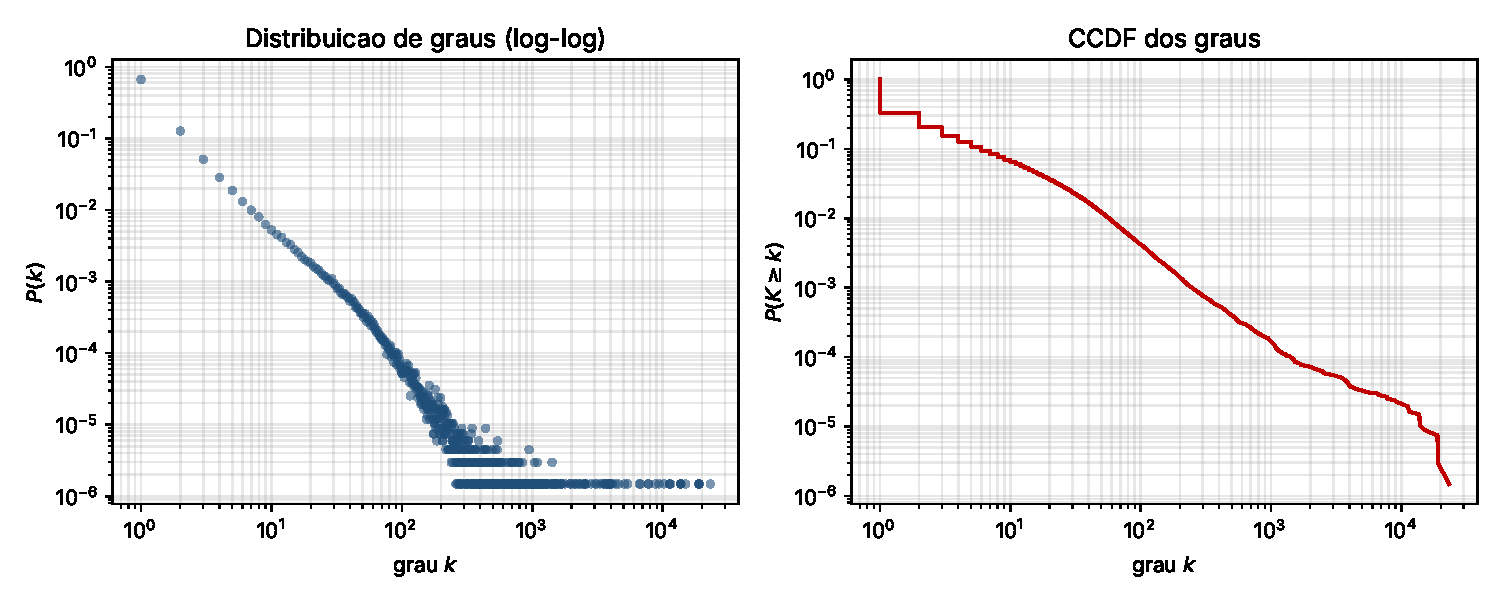
\includegraphics[width=0.95\textwidth]{../figuras/fig_graus.pdf}
\caption{Distribuição de graus em escala log-log (esquerda) e distribuição
acumulada complementar --- CCDF (direita).}
\label{fig:graus}
\end{figure*}

\paragraph{Comentário.} Em escala log-log a distribuição é aproximadamente
retilínea ao longo de três ordens de grandeza, com um ``ombro'' nos graus
baixos. \fracGrauUm{}\% dos sites têm grau exatamente~1 e
\fracGrauAteDois{}\% têm grau no máximo~2: a esmagadora maioria aparece
uma ou duas vezes no mês e desaparece. No outro extremo,
\texttt{\hubPrimeiro{}} atinge grau \hubPrimeiroGrau{}. A Seção~\ref{sec:leipotencia} quantifica a cauda.

\subsection{Componentes conexas}

\begin{figure}[t]
\centering
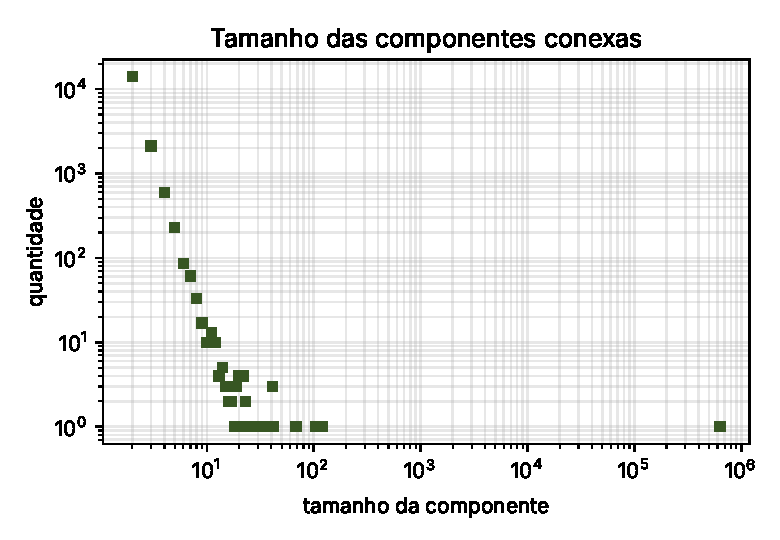
\includegraphics[width=0.52\columnwidth]{../figuras/fig_componentes.pdf}
\caption{Distribuição dos tamanhos das componentes conexas.}
\label{fig:componentes}
\end{figure}

\paragraph{Comentário.} São \numComponentes{} componentes, mas a
distribuição é tão desbalanceada quanto a dos graus: a maior contém
\tamCG{} vértices (\fracCG{}\% do total) e \fracArestasCG{}\% das arestas;
a segunda tem apenas \segundaComp{} e a terceira \terceiraComp{}.
São \compMenoresDez{} componentes com menos de dez vértices, das quais
\compDois{} são pares isolados --- tipicamente um blog obscuro que, no mês
observado, só trocou link com um único outro site. Não há vértices
isolados, pois o grafo foi construído a partir das arestas.

\subsection{Distâncias}

\begin{figure}[t]
\centering
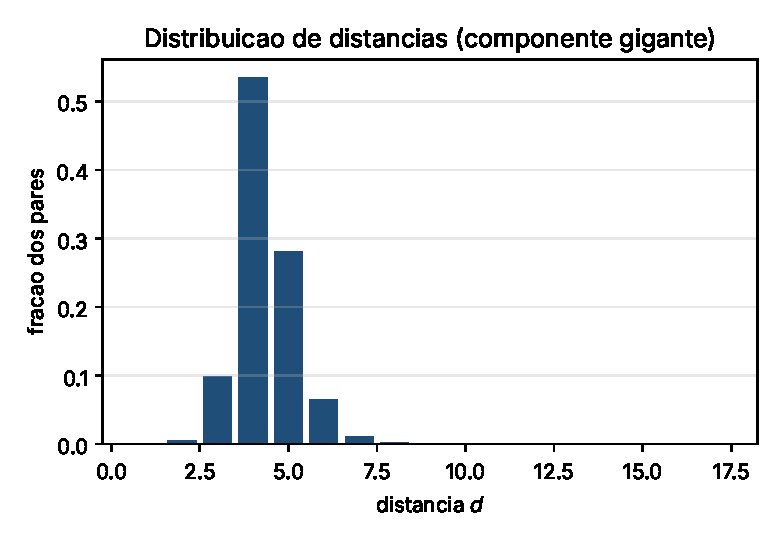
\includegraphics[width=0.52\columnwidth]{../figuras/fig_distancias.pdf}
\caption{Distribuição das distâncias na componente gigante
(amostra de \caminhoMedioFontes{} fontes).}
\label{fig:distancias}
\end{figure}

\paragraph{Comentário.} A distribuição é fortemente concentrada: a maior
parte dos pares está a distância 4 ou 5, com média \caminhoMedio{}, ao
passo que o diâmetro é \diametro{} e o raio é \raio{}. Em outras palavras,
existem caminhos longos, mas eles são raríssimos --- cauda da distribuição,
não o seu corpo. Para um grafo com mais de seiscentos mil vértices, um
caminho médio pouco acima de quatro é notável e já antecipa o resultado da
Seção~\ref{sec:smallworld}.

\subsection{Sites mais centrais e visualização}

\begin{table}[t]
\centering
\caption{Quinze sites de maior grau na rede.}
\label{tab:hubs}
\small
\begin{tabular}{rlr}
\hline
\# & \textbf{Site (\textit{hostname})} & \textbf{Grau} \\ \hline
1 & \texttt{blogger.com} & 23\,196 \\
2 & \texttt{4.bp.blogspot.com} & 19\,099 \\
3 & \texttt{1.bp.blogspot.com} & 19\,076 \\
4 & \texttt{2.bp.blogspot.com} & 18\,942 \\
5 & \texttt{3.bp.blogspot.com} & 18\,906 \\
6 & \texttt{en.wikipedia.org} & 14\,992 \\
7 & \texttt{bp3.blogger.com} & 13\,822 \\
8 & \texttt{bp2.blogger.com} & 13\,784 \\
9 & \texttt{bp1.blogger.com} & 13\,750 \\
10 & \texttt{bp0.blogger.com} & 13\,736 \\
11 & \texttt{presearch.oops.jp} & 11\,489 \\
12 & \texttt{sulit.com.ph} & 11\,324 \\
13 & \texttt{wordlank.mods.jp} & 11\,280 \\
14 & \texttt{mixfind.whitesnow.jp} & 10\,230 \\
15 & \texttt{nnseek.com} & 9\,397 \\
\hline
\end{tabular}

\end{table}

\begin{figure}[t]
\centering
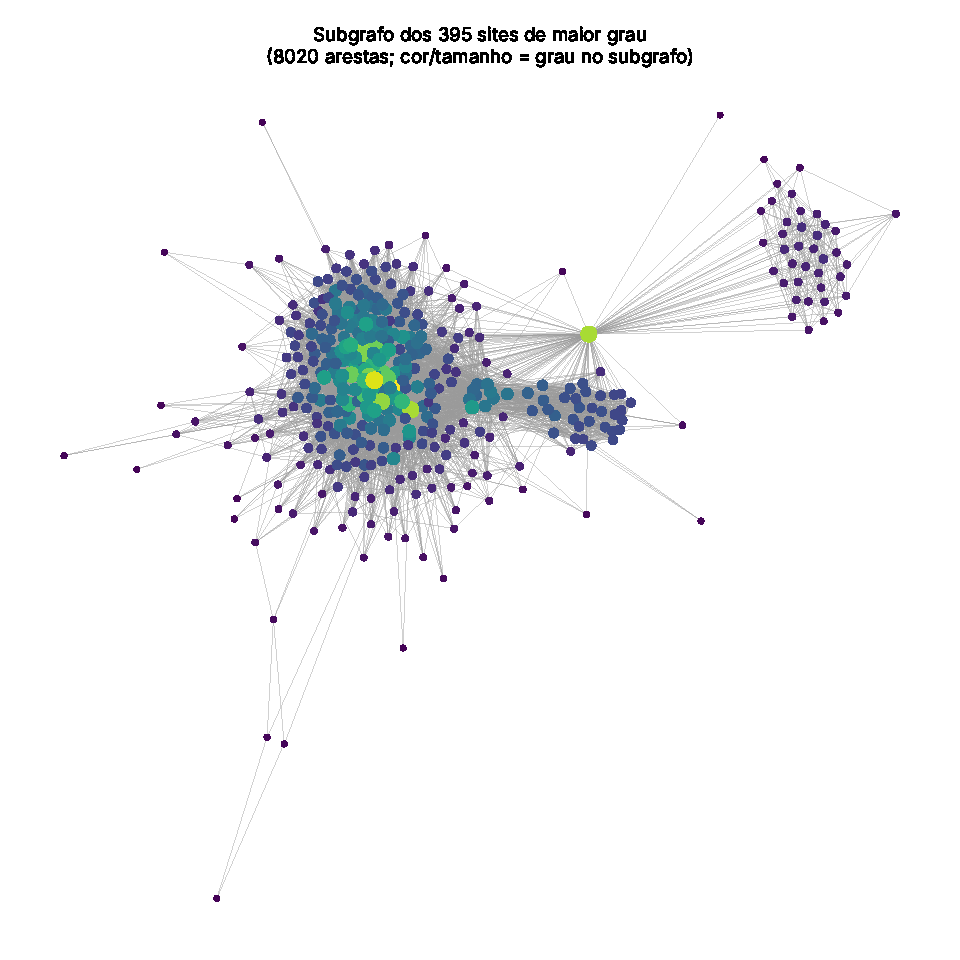
\includegraphics[width=0.74\columnwidth]{../figuras/fig_visualizacao.pdf}
\caption{Visualização reduzida: subgrafo induzido pelos 400 sites de maior
grau da componente gigante, com disposição de Fruchterman--Reingold.
Dos 400, os 395 que mantêm ao menos uma aresta \emph{dentro} do subgrafo
são desenhados (os 5 restantes só se ligam a sites de fora dele). Cor e
tamanho codificam o grau dentro do subgrafo.}
\label{fig:visualizacao}
\end{figure}

\paragraph{Comentário.} A visualização mostra um núcleo denso
fortemente interconectado, cercado por uma periferia que se liga ao núcleo
por poucas arestas --- a estrutura ``núcleo-periferia'' típica de redes de
hiperlinks. O conteúdo da Tabela~\ref{tab:hubs} é discutido na
Seção~\ref{sec:descoberta}, pois é a descoberta mais interessante deste
trabalho.

% =====================================================================
\section{Parte II --- Algoritmos da disciplina}
\label{sec:parte2}

\subsection{Protocolo de medição}

Cada algoritmo foi executado $T$ vezes sobre a componente gigante
($n=\tamCG{}$, $m=\arestasCG{}$). Para os algoritmos com fonte única
(BFS, DFS, Dijkstra, Prim) sorteou-se uma fonte diferente a cada repetição,
de modo que a variância medida não dependa de um vértice particular.
Reporta-se média, desvio padrão amostral e intervalo de confiança de 95\%,
usando a distribuição \textbf{Normal} quando $T\geq30$ e a
\textbf{$t$-Student} quando $T<30$, conforme o enunciado:
\[
\bar{x} \pm z_{\alpha/2}\frac{\sigma}{\sqrt{n}}
\quad (n \geq 30), \qquad
\bar{x} \pm t_{\alpha/2}\frac{\sigma}{\sqrt{n}}
\quad (n < 30,\ \sigma \text{ desconhecido}).
\]

\paragraph{Pesos.} Os algoritmos de caminho mínimo e de árvore geradora
precisam de custos. Como o peso bruto de uma aresta é o \emph{número de
hiperlinks} entre dois sites (quanto maior, mais forte o laço), adotou-se
$c(u,v) = 1/\text{peso}(u,v)$: ligações mais frequentes ficam ``mais
curtas''. A árvore geradora mínima é, portanto, a árvore que maximiza a
afinidade acumulada entre os sites.

\subsection{Complexidade teórica das implementações}
\label{sec:complexidade}

As cotas abaixo não são citadas de fora: elas decorrem do código que
acompanha este trabalho (\texttt{scripts/lib\_algoritmos.py}). Em todas,
$n = |V|$ e $m = |E|$, e o grafo está em formato CSR --- dois vetores,
\texttt{indptr} e \texttt{indices}, em que a vizinhança de $v$ ocupa as
posições \texttt{indptr[v]} a \texttt{indptr[v+1]}. Logo percorrer a
vizinhança de $v$ custa $\Theta(\mathrm{grau}(v))$ e
$\sum_v \mathrm{grau}(v) = 2m$. A montagem do CSR em si custa
$O(m\log m)$, dominada pela ordenação das arestas.

\paragraph{BFS --- $\Theta(n+m)$.} A fila é uma lista com índice de
cabeça, nunca \texttt{pop(0)}, de modo que desenfileirar é $O(1)$. O teste
\texttt{dist[v] < 0} garante que cada vértice entra na fila uma única vez,
dando $n$ enfileiramentos. Ao desenfileirar $u$, o laço percorre
exatamente $\mathrm{grau}(u)$ posições do CSR; somando sobre todos os
vértices, $2m$ inspeções de aresta. Total: $\Theta(n+m)$ em tempo e
$\Theta(n)$ em memória.

\paragraph{DFS --- $\Theta(n+m)$.} A pilha é explícita, e o vetor
\texttt{ponteiro[u]} guarda em que ponto do CSR a varredura de $u$ parou.
Esse detalhe é o que garante a cota: sem ele, cada retorno de $u$ ao topo
da pilha recomeçaria a varredura do início da sua lista de adjacência, e
o custo degeneraria para $O(n\cdot m)$. Com o ponteiro, cada aresta é
inspecionada no máximo uma vez por extremidade e cada vértice entra e sai
da pilha uma vez: $\Theta(n+m)$.

\paragraph{Verificação de eulerianidade --- $\Theta(n)$.} Uma única
passada sobre o vetor de graus contando os ímpares. A conexidade, segunda
condição do teorema de Euler, já foi estabelecida pela BFS que extraiu a
componente.

\paragraph{Dijkstra --- $O((n+m)\log n)$.} O \texttt{heapq} de Python é um
heap binário e não oferece \textit{decrease-key}; a implementação usa
remoção preguiçosa, empurrando uma nova entrada a cada relaxamento bem
sucedido e descartando as obsoletas pelo vetor \texttt{fechado}. Cada
aresta pode gerar no máximo uma inserção por sentido, logo no máximo $2m$
inserções, mais a inicial. O heap nunca passa de $2m+1$ entradas, e cada
inserção ou remoção custa $O(\log m)$. Como o grafo é simples,
$m \leq n^2$ e portanto $\log m \leq 2\log n$. Total:
$O((n+m)\log n)$, com memória $O(n+m)$.

\paragraph{Bellman--Ford --- $O(n\cdot m)$.} São $n-1$ iterações, cada uma
relaxando as $m$ arestas nos dois sentidos, mais uma passada final de
$O(m)$ para detectar ciclo negativo. O laço é interrompido quando uma
passada inteira não produz relaxamento; sendo $d$ o número de camadas de
distância a partir da fonte, o custo real é $O(d\cdot m)$. Em uma rede de
mundo pequeno $d$ é pequeno, e é daí que vem o expoente observado
$\mathbf{\expBF}$ da Tabela~\ref{tab:expoentes}, abaixo de~1.

\paragraph{Floyd--Warshall --- $\Theta(n^3)$ em tempo, $\Theta(n^2)$ em
memória.} Três laços aninhados sobre $k$, $i$ e $j$, cada um com $n$
iterações, sobre uma matriz $n \times n$. O teste
\texttt{if dik == inf: continue} descarta linhas inteiras quando $i$ não
alcança $k$, o que ajuda em grafos esparsos mas não altera o pior caso.
A memória quadrática é a restrição mais severa: para a componente gigante
seriam \fwMemoria.

\paragraph{Tarjan (SCC e articulações) --- $\Theta(n+m)$.} Ambas as
variantes são uma DFS com \textit{low-link}. Cada vértice recebe índice
de descoberta uma vez, cada aresta é inspecionada uma vez a partir de
cada extremidade, e cada vértice entra e sai da pilha de componentes
exatamente uma vez. O desempilhamento final é amortizado: ao longo de
toda a execução ele remove $n$ elementos no total.

\paragraph{Prim --- $O(m\log n)$.} Mesma estrutura de heap binário com
remoção preguiçosa usada no Dijkstra: no máximo $2m$ inserções, cada uma
$O(\log m) = O(\log n)$. Com um heap de Fibonacci a cota cairia para
$O(m + n\log n)$, mas a biblioteca padrão de Python não oferece essa
estrutura.

\paragraph{Kruskal --- $O(m\log m)$.} A ordenação das $m$ arestas por
custo domina o algoritmo. A seguir há $2m$ operações \texttt{find} e até
$n-1$ \texttt{union} sobre a estrutura união-busca, implementada com
compressão de caminho e união por \textit{rank}; essas operações somam
$O(m\,\alpha(n))$, com $\alpha$ a inversa da função de Ackermann, menor
que~5 para qualquer $n$ fisicamente realizável. O total é, portanto,
$O(m\log m) + O(m\,\alpha(n)) = O(m\log m)$.

\paragraph{\textit{BoundingDiameters} --- sem cota melhor que
$O(n\cdot m)$.} Vale registrar a honestidade aqui: o algoritmo que
fornece diâmetro e raio exatos é rápido por \emph{heurística de poda},
não por garantia assintótica. No pior caso ele executa uma BFS por
vértice, exatamente como a abordagem ingênua. O que ele garante é a
corretude; a eficiência é empírica, e neste grafo foi excelente ---
\bfsDiametro{} BFS em vez de \tamCG{}.

\subsection{Tempos de execução}

\begin{table*}[t]
\centering
\caption{Tempo real de execução das implementações próprias.
$^{\dagger}$ Bellman--Ford foi executado sobre um subgrafo induzido com
$n=\subBF{}$ e $m=\subBFm{}$.
$^{\ddagger}$ Floyd--Warshall sobre um subgrafo com $n=\subFW{}$.}
\label{tab:tempos}
\scriptsize
\begin{tabular}{lccrrrc}
\hline
\textbf{Algoritmo} & \textbf{Complexidade} & $T$ & \textbf{Média (s)} & \textbf{DP (s)} & \textbf{IC 95\% (s)} & \textbf{Dist.} \\ \hline
Busca em largura (BFS) & $O(n+m)$ & 30 & 1,0093 & 0,1883 & [0,9419; 1,0766] & Z \\
Busca em profundidade (DFS) & $O(n+m)$ & 30 & 0,8758 & 0,1073 & [0,8375; 0,9142] & Z \\
Verificação de eulerianidade & $O(n)$ & 30 & 0,0191 & 0,0001 & [0,0191; 0,0192] & Z \\
Dijkstra (fila de prioridade) & $O((n+m)\log n)$ & 30 & 2,9532 & 0,2367 & [2,8685; 3,0379] & Z \\
Bellman--Ford$^{\dagger}$ & $O(n\cdot m)$ & 10 & 0,0153 & 0,0002 & [0,0152; 0,0154] & $t$ \\
Floyd--Warshall$^{\ddagger}$ & $O(n^3)$ & 10 & 2,0143 & 0,0768 & [1,9594; 2,0692] & $t$ \\
Floyd--Warshall (NumPy)$^{\ddagger}$ & $O(n^3)$ & 10 & 0,1535 & 0,0060 & [0,1492; 0,1577] & $t$ \\
Tarjan (comp.\ fortemente conexas) & $O(n+m)$ & 10 & 1,3101 & 0,0868 & [1,2480; 1,3721] & $t$ \\
Tarjan (articulações e pontes) & $O(n+m)$ & 10 & 1,8570 & 0,1906 & [1,7206; 1,9933] & $t$ \\
Prim (AGM) & $O(m\log n)$ & 30 & 9,8165 & 0,4012 & [9,6730; 9,9601] & Z \\
Kruskal (AGM) & $O(m\log m)$ & 10 & 3,6038 & 0,1873 & [3,4698; 3,7378] & $t$ \\
\hline
\end{tabular}

\end{table*}

\paragraph{Comentário.} Os algoritmos lineares e quase lineares percorrem
a componente gigante inteira em poucos segundos. Dois algoritmos
\textbf{não} cabem no grafo completo e precisaram de subgrafos:

\begin{itemize}[nosep]
  \item \textbf{Bellman--Ford}, $O(n\cdot m)$, exigiria
        $\approx 10^{12}$ relaxamentos. Vale observar que ele é
        \emph{desnecessário} aqui: não há pesos negativos (todos os custos
        são $1/\text{peso} > 0$), de modo que Dijkstra resolve o mesmo
        problema em tempo quase linear. Bellman--Ford só se justificaria se
        houvesse arestas de custo negativo --- ele foi incluído por ser
        parte do enunciado e para medir empiricamente o custo $O(nm)$.
  \item \textbf{Floyd--Warshall}, $O(n^3)$ em tempo e $O(n^2)$ em memória,
        precisaria de $2{,}5\times10^{17}$ operações e de uma matriz de
        $3{,}2$~TB. Ele foi executado em um subgrafo de \subFW{} vértices,
        o suficiente para medir o expoente empírico.
\end{itemize}

\subsection{Complexidade teórica \textit{vs.} observada}

Para cada algoritmo mediu-se o tempo em subgrafos induzidos de tamanho
crescente (obtidos por BFS a partir de uma semente, o que garante
conexidade) e ajustou-se, por mínimos quadrados em escala log-log, o modelo
$t \propto x^{b}$, onde $x$ é a variável de custo teórica. Se a
implementação respeita a complexidade esperada, $b \approx 1$.

\begin{table}[t]
\centering
\caption{Expoente empírico $b$ em $t\propto x^{b}$.}
\label{tab:expoentes}
\small
\begin{tabular}{llcc}
\hline
\textbf{Algoritmo} & \textbf{Variável de custo $x$} & $b$ \textbf{teórico} & $b$ \textbf{observado} \\ \hline
BFS & $n+m$ & 1,00 & 1,167 \\
DFS & $n+m$ & 1,00 & 1,140 \\
Dijkstra & $(n+m)\log n$ & 1,00 & 1,178 \\
Prim & $m\log n$ & 1,00 & 1,264 \\
Kruskal & $m\log m$ & 1,00 & 1,061 \\
Tarjan & $n+m$ & 1,00 & 1,182 \\
Bellman--Ford & $n\cdot m$ & 1,00 & 0,716 \\
Floyd--Warshall & $n^3$ & 1,00 & 0,981 \\
\hline
\end{tabular}

\end{table}

\begin{figure*}[t]
\centering
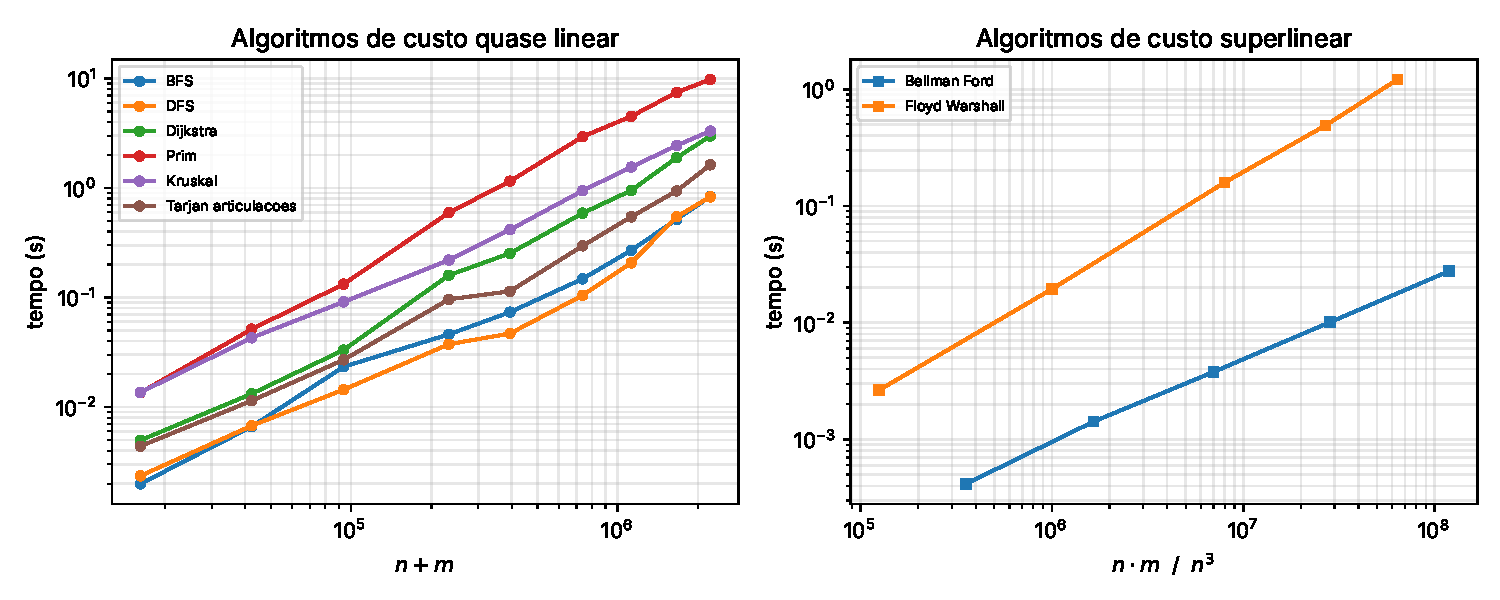
\includegraphics[width=0.95\textwidth]{../figuras/fig_escalabilidade.pdf}
\caption{Tempo real \textit{vs.} variável de custo teórica, em escala
log-log. Esquerda: algoritmos de custo quase linear. Direita: algoritmos
superlineares.}
\label{fig:escalabilidade}
\end{figure*}

\paragraph{Comentário.} Os expoentes ficam próximos de~1, confirmando que
as implementações atingem a complexidade esperada. Os desvios têm
explicação concreta: em grafos pequenos o custo fixo do interpretador
domina (o que puxa $b$ para baixo), e nos maiores a localidade de cache
piora (o que puxa $b$ para cima). O caso mais instrutivo é o do
Bellman--Ford, cujo expoente observado fica \emph{abaixo} de~1: a
implementação interrompe o laço quando uma passada não produz relaxamento,
e como o diâmetro do grafo é pequeno (\diametro{}), bastam poucas passadas
--- o pior caso $O(nm)$ simplesmente não ocorre em redes de mundo pequeno.

\subsection{Eulerianidade}

A verificação é imediata: um grafo não dirigido conexo admite circuito
euleriano se e somente se todos os seus vértices têm grau par, e admite
trilha euleriana aberta se e somente se exatamente dois vértices têm grau
ímpar. A componente gigante tem \grauImpar{} vértices de grau ímpar
(\fracGrauImpar{}\% do total). Logo o grafo \textbf{não é euleriano nem
semi-euleriano}. Isso era esperado: a paridade dos graus é uma condição
aritmética muito restritiva, que nenhuma rede real não planejada satisfaz.

\subsection{Tarjan: componentes fortemente conexas, articulações e pontes}
\label{sec:tarjan}

O algoritmo de Tarjan foi aplicado em duas variantes.

\paragraph{(a) Componentes fortemente conexas.} Sobre o grafo
\textbf{dirigido} original (\nDirigido{} vértices, \mDirigido{} arestas),
obtêm-se \numSCC{} componentes fortemente conexas, das quais \sccTriviais{}
são triviais (um único vértice). A maior tem \maiorSCC{} vértices, apenas
\fracSCC{}\% do grafo. O contraste com a conectividade \emph{fraca}
(\fracCG{}\% em uma única componente) é expressivo e revela a assimetria
da rede: quase todo mundo está ligado a quase todo mundo se ignorarmos a
direção dos links, mas o ``núcleo'' em que é possível ir e voltar é
pequeno. Grandes veículos de mídia recebem muitos links e devolvem poucos,
o que os deixa fora do núcleo fortemente conexo --- é a estrutura de
``gravata-borboleta'' descrita por Broder et al.\ para a Web
\cite{broder2000}.

\paragraph{(b) Vértices de articulação e pontes.} Na componente gigante há
\numArticulacoes{} vértices de articulação (\fracArticulacoes{}\% dos
vértices) e \numPontes{} pontes. Cada um desses vértices, se removido,
quebra a rede em pedaços --- resultado que dialoga diretamente com a
análise de robustez da Seção~\ref{sec:robustez}.

\subsection{Árvore geradora mínima}

Prim e Kruskal produziram o mesmo custo total, \custoMST{} (as duas
implementações concordam até a décima segunda casa decimal; a diferença
residual é acúmulo de erro de ponto flutuante, já que as arestas são
somadas em ordens diferentes), com \arestasMST{} arestas ($=n-1$, como esperado em grafo conexo). A
coincidência numérica entre as duas implementações é também uma verificação
cruzada. Vale registrar uma diferença conceitual observada durante a
validação: Prim, partindo de uma fonte, devolve a árvore geradora mínima
\emph{da componente que contém a fonte}, enquanto Kruskal devolve a
\textbf{floresta} geradora mínima de todo o grafo. Na componente gigante,
conexa por construção, os dois coincidem.

% =====================================================================
\section{Parte III --- Análise estrutural}
\label{sec:parte3}

\subsection{O grafo é um mundo pequeno?}
\label{sec:smallworld}

\paragraph{Critério.} Um grafo $G$ é mundo pequeno quando
$L(G) \approx L_{\text{aleatório}}$ e
$C(G) \gg C_{\text{aleatório}}$. Implementou-se do zero: o coeficiente de
clusterização local (contagem de triângulos por interseção de listas de
adjacência), o comprimento médio por BFS amostrada, um gerador
Erdős--Rényi $G(n,m)$ e um modelo de configuração obtido por
\textbf{\swTrocas{} trocas duplas de arestas} aceitas sobre o próprio
grafo, que preserva exatamente a sequência de graus.

\begin{table*}[t]
\centering
\caption{Mundo pequeno: grafo real \textit{vs.} modelos nulos.
$C$ estimado em \swAmostraC{} vértices, $L$ em \swAmostraL{} fontes
(IC 95\% de $L$ no grafo real: $[\swLICa{};\,\swLICb{}]$). O valor de
$C$ para Erdős--Rényi é tão pequeno que a estimativa por amostragem é
ruidosa (IC 95\%: $[\swCerICa{};\,\swCerICb{}]$); ele é consistente com
o valor analítico $\langle k\rangle/n = \swCanalitico{}$, que daria
$C/C_r = \swRazaoCanalitico{}$ em vez de \swRazaoCer{} --- a mesma ordem
de grandeza.}
\label{tab:smallworld}
\small
\begin{tabular}{lccc}
\hline
 & \textbf{G106 (real)} & \textbf{Erdős--Rényi $G(n,m)$} &
 \textbf{Configuração} \\ \hline
$C$                     & \swC{}  & \swCer{}  & \swCconf{} \\
$L$                     & \swL{}  & \swLer{}  & \swLconf{} \\
$C/C_{r}$               & ---     & \swRazaoCer{} & \swRazaoCconf{} \\
$L/L_{r}$               & ---     & \swRazaoLer{} & \swRazaoLconf{} \\
$\sigma=(C/C_r)/(L/L_r)$& ---     & \swSigmaEr{}  & \swSigmaConf{} \\
\hline
\end{tabular}
\end{table*}

\begin{figure*}[t]
\centering
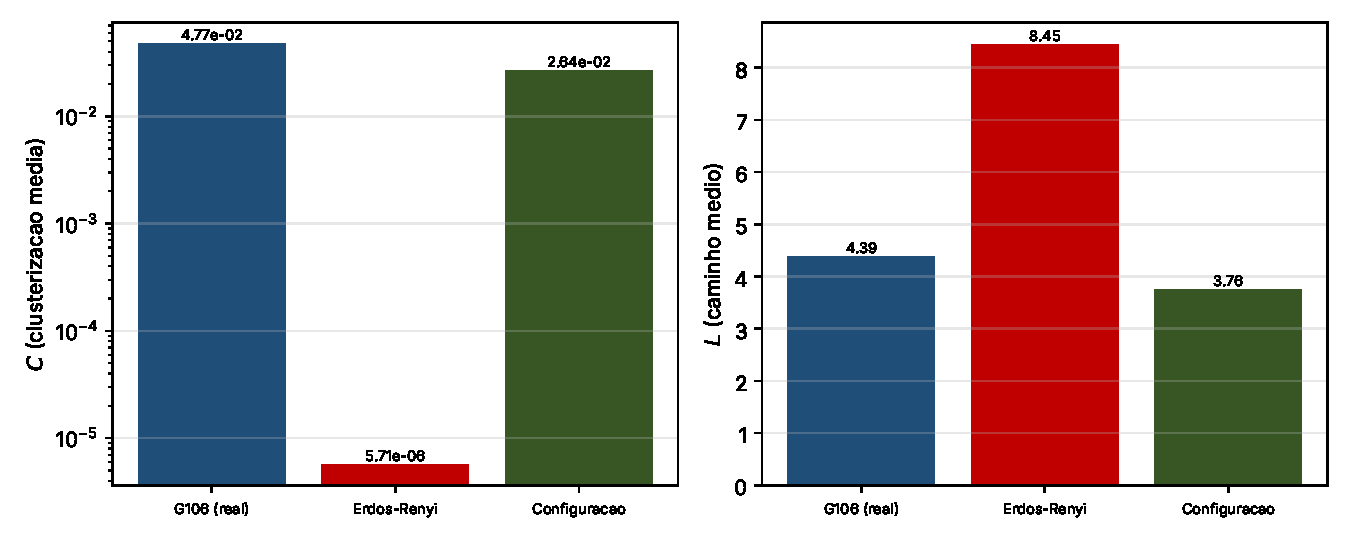
\includegraphics[width=0.85\textwidth]{../figuras/fig_small_world.pdf}
\caption{Clusterização (escala logarítmica) e caminho médio do grafo real
comparados aos dois modelos nulos.}
\label{fig:smallworld}
\end{figure*}

\paragraph{Resposta: sim --- e de forma ainda mais forte do que o
critério exige.} A segunda condição do Apêndice~A é satisfeita com enorme
folga: a clusterização real é \swRazaoCer{} vezes a do grafo aleatório
equivalente. Quanto à primeira, o caminho médio real (\swL{}) não é apenas
da mesma \emph{ordem} do aleatório (\swLer{}): é cerca de metade dele
($L/L_r = \swRazaoLer{}$). Isso não enfraquece o diagnóstico --- reforça-o.
Redes com expoente $2<\gamma<3$, como esta
(Seção~\ref{sec:leipotencia}), são \emph{mundos ultrapequenos}: os
\textit{hubs} encurtam as distâncias para além do que um grafo aleatório
homogêneo consegue, de modo que $L$ cresce como $\ln\ln n$ em vez de
$\ln n$. O valor analítico para o grafo aleatório,
$L_{rand}\approx\ln n/\ln\langle k\rangle = \swLanalitico{}$, confirma o
valor simulado, assim como $C_{rand}\approx\langle k\rangle/n =
\swCanalitico{}$. Com $\sigma = \swSigmaEr{} \gg 1$, o grafo é um mundo
pequeno sem qualquer ambiguidade.

\paragraph{O teste contra o modelo de configuração.} Esse segundo modelo
nulo é bem mais severo, pois preserva \emph{exatamente} a sequência de
graus --- e portanto todos os \textit{hubs} --- randomizando apenas a
forma como as pontas de aresta se emparelham. O resultado é mais sóbrio e
mais informativo que a comparação com Erdős--Rényi:

\begin{itemize}[nosep]
  \item o \textbf{caminho curto} é inteiramente explicado pela sequência
        de graus: o modelo de configuração chega a $L_{conf}=\swLconf{}$,
        \emph{menor} ainda que o real ($L/L_{conf} = \swRazaoLconf{}$).
        Não há nada de especial na topologia além dos graus que torne este
        grafo mais ``curto'';
  \item o \textbf{agrupamento local} é em boa parte, mas não
        inteiramente, explicado pelos graus: a clusterização cai de
        \swC{} para \swCconf{}, isto é, $C/C_{conf} = \swRazaoCconf{}$.
        Sobra um excesso real de aproximadamente 80\%, com
        $\sigma_{conf} = \swSigmaConf{} > 1$.
\end{itemize}

\noindent
A leitura honesta, portanto, é esta: comparado a um grafo \emph{homogêneo}
o G106 é um mundo pequeno espetacular; comparado a um grafo com a
\emph{mesma heterogeneidade de graus}, ele continua sendo um mundo
pequeno, mas o seu diferencial encolhe para um excesso moderado de
triângulos. Boa parte do que normalmente se atribui à ``propriedade de
mundo pequeno'' de redes reais é, na verdade, consequência direta da cauda
pesada da distribuição de graus --- e só a comparação com o modelo de
configuração torna isso visível.

\paragraph{Faz sentido para este grafo?} Faz, e por um mecanismo
identificável. Blogs e veículos de mídia linkam preferencialmente quem já
está no seu círculo temático ou regional, o que gera triângulos
(se $A$ linka $B$ e $C$, é provável que $B$ e $C$ também se linkem).
Ao mesmo tempo, um punhado de \textit{hubs} globais --- plataformas de
blog, Wikipédia, grandes agências --- funciona como atalho entre
comunidades distantes, colapsando as distâncias. É exatamente a receita de
Watts e Strogatz \cite{watts1998}: agrupamento local alto mais poucos
atalhos de longo alcance.

\paragraph{Implicação prática.} Uma informação (um meme) precisa de
poucos saltos para atravessar toda a blogosfera: em média \swL{} e no
pior caso \diametro{}. Isso explica a velocidade com que uma frase
atravessa o ecossistema de notícias --- o fenômeno que o próprio
\textit{Memetracker} foi construído para medir \cite{leskovec2009}.
O reverso também vale: desinformação se espalha igualmente rápido, e
estratégias de contenção baseadas em ``bloquear a propagação
gradualmente'' são pouco eficazes em uma rede com esse diâmetro.

\subsection{A distribuição de graus sugere uma lei de potência?}
\label{sec:leipotencia}

Seguiu-se o protocolo de Clauset, Shalizi e Newman \cite{clauset2009}:
estimação de $\gamma$ por máxima verossimilhança para cada $k_{min}$
candidato, escolha do $k_{min}$ que minimiza a distância de
Kolmogorov--Smirnov, teste de bondade do ajuste por \textit{bootstrap}
semiparamétrico e comparação com alternativas por razão de verossimilhança.

\begin{table}[t]
\centering
\caption{Ajuste de lei de potência à cauda da distribuição de graus.}
\label{tab:leipotencia}
\small
\begin{tabular}{lr}
\hline
\textbf{Parâmetro} & \textbf{Valor} \\ \hline
$k_{min}$ ótimo (menor KS)                      & \plKmin{} \\
Expoente $\gamma$ (máxima verossimilhança)      & $\plGamma \pm \plGammaErro$ \\
Vértices na cauda                               & \plNcauda{} (\plFracCauda{}\% dos vértices) \\
Distância KS                                    & \plKS{} \\
Valor-$p$ do \textit{bootstrap} (\plBoot{} amostras) & \plPvalor{} \\
$\gamma$ por mínimos quadrados no log-log       & \plGammaOLS{} ($R^2=\plROLS{}$) \\
\hline
\end{tabular}
\end{table}

\begin{figure*}[t]
\centering
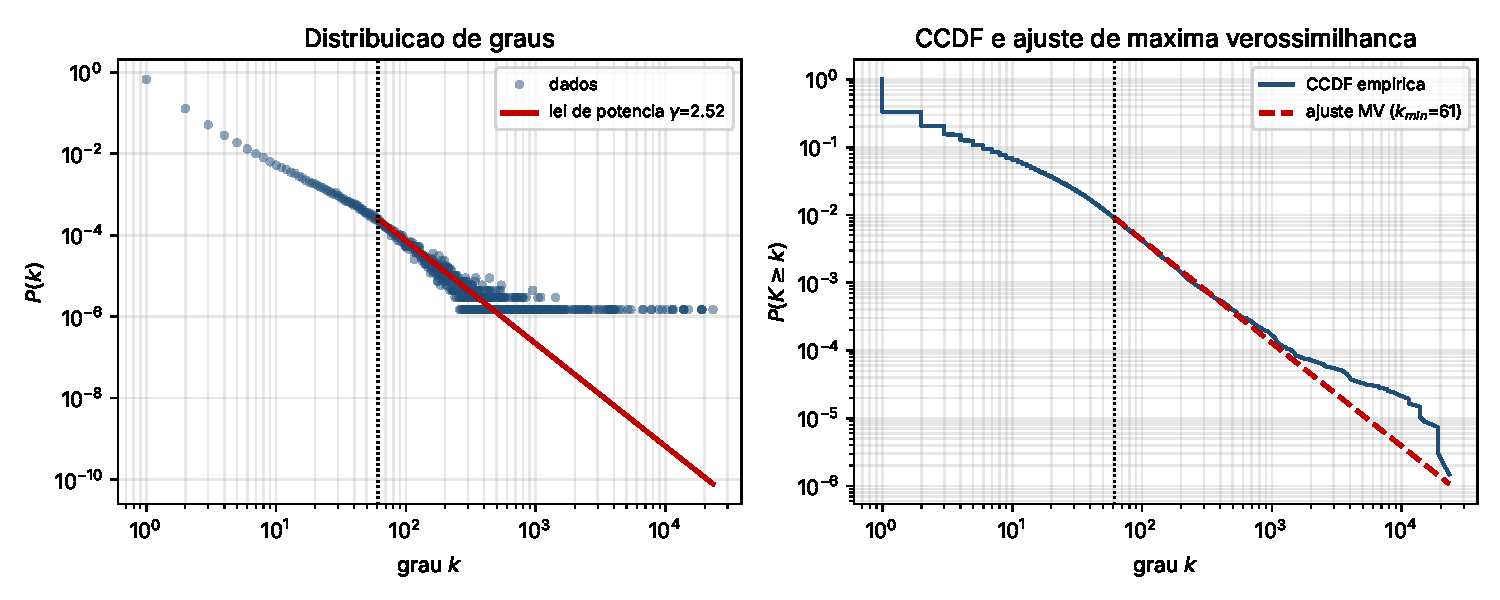
\includegraphics[width=0.95\textwidth]{../figuras/fig_lei_potencia.pdf}
\caption{Esquerda: distribuição de graus e lei de potência ajustada.
Direita: CCDF empírica e ajuste de máxima verossimilhança acima de
$k_{min}=\plKmin{}$.}
\label{fig:leipotencia}
\end{figure*}

\begin{figure}[t]
\centering
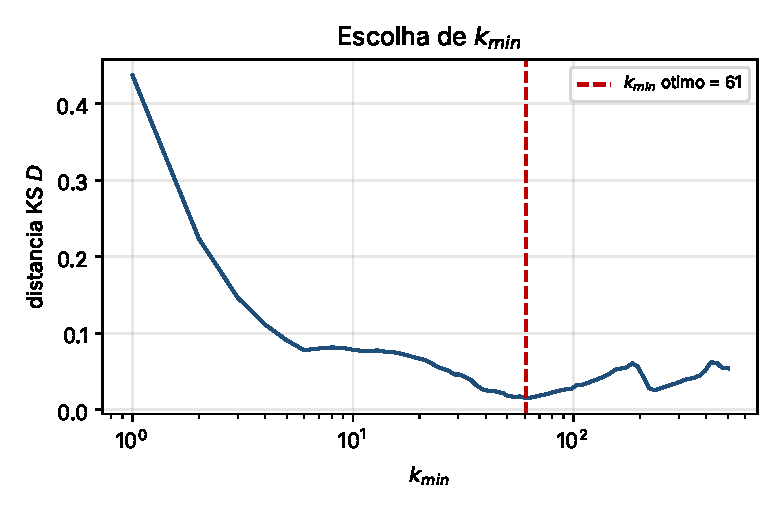
\includegraphics[width=0.52\columnwidth]{../figuras/fig_kmin.pdf}
\caption{Distância de Kolmogorov--Smirnov em função de $k_{min}$;
o mínimo define o início da cauda.}
\label{fig:kmin}
\end{figure}

\paragraph{Resposta: sim no comportamento, não no sentido estrito.} A
cauda é inequivocamente pesada e $\gamma = \plGamma$ cai exatamente na
faixa $2<\gamma<3$ observada na maioria das redes reais, em que a média do
grau é finita mas a variância diverge --- o que já havíamos detectado
empiricamente ($\sigma/\mu\approx17$). Por outro lado, o teste formal
rejeita a hipótese de lei de potência \emph{pura}
($p=\plPvalor{} < 0{,}10$). Isso é a norma, não a exceção: com
\plNcauda{} pontos na cauda, o teste KS detecta desvios minúsculos, e
praticamente nenhuma rede empírica passa no teste estrito de
\cite{clauset2009}. A leitura correta é: \emph{a cauda é pesada e
compatível com lei de potência na faixa ajustada, mas não é exatamente uma
lei de potência pura em todo o intervalo}.

\paragraph{Sobre o ajuste por mínimos quadrados.} O ajuste ingênuo da reta
no log-log dá $\gamma = \plGammaOLS{}$ com $R^2 = \plROLS{}$ --- um valor
não só diferente como \emph{impossível}, já que uma lei de potência com
$\gamma\leq1$ não é normalizável. É uma demonstração prática do viés
denunciado por \cite{clauset2009}: regredir frequências em escala log-log
dá peso igual a pontos da cauda, que são estimados com pouquíssimas
amostras. O estimador de máxima verossimilhança é o correto.

\paragraph{Comparação com alternativas.} A exponencial é descartada com
folga (razão de verossimilhança $\plLRexp{}$ a favor da lei de potência).
Já a log-normal truncada empata: o seu estimador de máxima verossimilhança
\emph{foge} para $\mu\to-\infty$, $\sigma\to+\infty$, limite em que a
log-normal converge para a própria lei de potência. A razão de verossimilhança resultante
(\plLRlognormal{}) é minúscula diante dos \plNcauda{} pontos da cauda, e
nesse regime os dois modelos deixam de ser distinguíveis: o teste de
Vuong, que pressupõe modelos não aninhados, perde validade. Conclusão honesta: os dados
distinguem claramente ``cauda pesada'' de ``cauda leve'', mas não
distinguem lei de potência de log-normal.

\subsection{O grafo é robusto?}
\label{sec:robustez}

Seguindo o Apêndice~C, trabalhou-se na componente gigante, com
$n=\tamCG{}$ e $r=\lfloor 0{,}05n\rfloor = \robR{}$ vértices removidos.
A remoção aleatória foi repetida $T=\robT{}$ vezes. O ataque dirigido
usou \textbf{ranking fixo por grau} (recomendado no enunciado) e, como
segunda centralidade, \textbf{PageRank}. A \textbf{intermediação}, a
outra opção recomendada no enunciado, exige o algoritmo de Brandes, de
custo $O(n\cdot m)\approx10^{12}$ operações neste grafo; ela é tratada
separadamente na Seção~\ref{sec:betweenness}, por amostragem de pivôs.

\begin{table*}[t]
\centering
\caption{Métricas após a remoção de \robR{} vértices (5\%).}
\label{tab:robustez}
\scriptsize
\begin{tabular}{lrrrr}
\hline
\textbf{Métrica} & \textbf{Intacto} & \textbf{Aleatório ($\mu\pm\sigma$)} & \textbf{Ataque: grau} & \textbf{Ataque: PageRank} \\ \hline
A --- maior componente & 632\,117 & 580\,480 $\pm$ 4270,7 & 38\,937 & 26\,623 \\
A --- $S$ (fração de $n$) & 1,0000 & 0,9183 $\pm$ 0,0068 & 0,0616 & 0,0421 \\
B --- n\textsuperscript{o} de componentes & 1 & 19\,014 $\pm$ 4050,5 & 470\,352 & 485\,823 \\
C --- caminho médio & 4,336 & 4,350 $\pm$ 0,0440 & 34,576 & 36,165 \\
C --- diâmetro & 21,0 & 20,7 $\pm$ 1,1725 & 85,0 & 110,0 \\
D --- fração de isolados & 0,0000 & 0,0307 $\pm$ 0,0066 & 0,7354 & 0,7592 \\
\hline
\end{tabular}

\end{table*}

\begin{figure}[t]
\centering
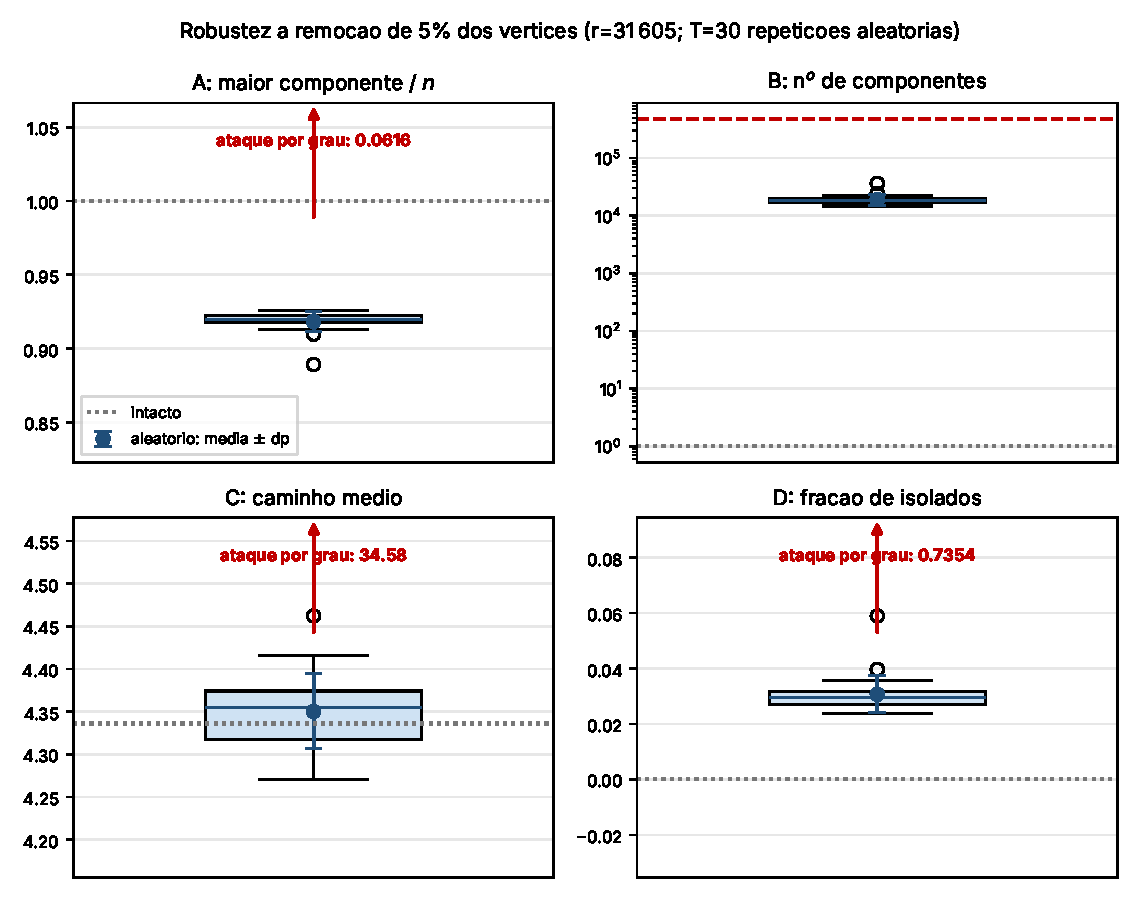
\includegraphics[width=0.78\columnwidth]{../figuras/fig_robustez_box.pdf}
\caption{\textit{Boxplots} das quatro métricas sob remoção aleatória
($T=\robT{}$ repetições), com média $\pm$ desvio padrão. A linha
pontilhada marca o grafo intacto; o valor do ataque dirigido por grau
aparece como linha tracejada vermelha quando cabe na escala e como seta
anotada quando está fora dela --- o que, por si só, já mostra a distância
entre os dois cenários.}
\label{fig:robustezbox}
\end{figure}

\begin{figure}[t]
\centering
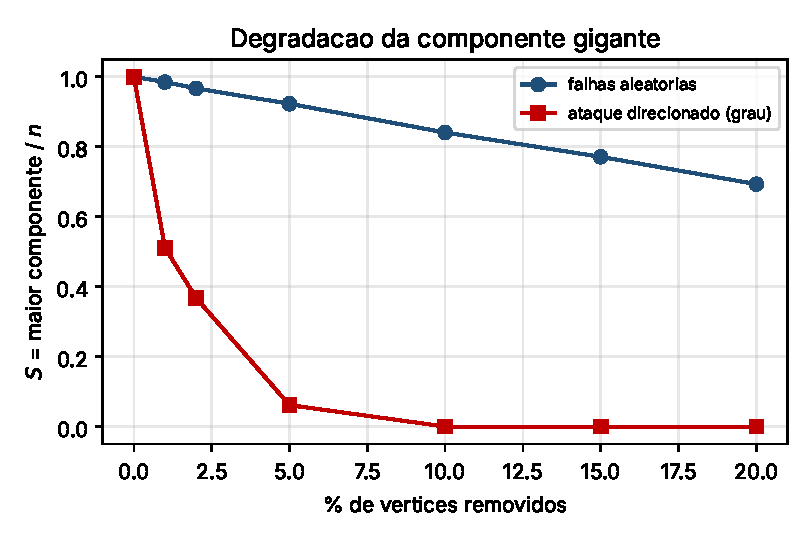
\includegraphics[width=0.55\columnwidth]{../figuras/fig_robustez_curva.pdf}
\caption{Fração $S$ da maior componente em função do percentual de
vértices removidos, por falha aleatória e por ataque dirigido.}
\label{fig:robustezcurva}
\end{figure}

\paragraph{Resposta: robusto a falhas, frágil a ataques.} Os números são
categóricos:

\begin{itemize}[nosep]
  \item \textbf{Remoção aleatória de 5\%:} a maior componente, que tinha
        \robSintacto{} vértices, passa a conter em média \robSrandAbs{}
        --- $S_{rand} = \robSrand{}$ dos vértices originais, com
        IC 95\% $=[\robSrandICa{};\,\robSrandICb{}]$; o número de
        componentes sobe de \robCompIntacto{} para \robCompRand{}; o
        caminho médio passa de \robLintacto{} para \robLrand{} e o
        diâmetro de \robDiamIntacto{} para \robDiamRand{}. A
        variabilidade entre as \robT{} repetições é mínima --- o desvio
        padrão de $S$ é \robSrandDP{} ---, o que mostra que o resultado não
        é sorte: a rede \emph{absorve} falhas aleatórias.
  \item \textbf{Ataque aos 5\% de maior grau:} $S_{cent} = \robScent{}$, o
        número de componentes salta para \robCompCent{}, o caminho médio da
        maior componente remanescente salta de \robLintacto{} para
        \robLcent{} e o seu diâmetro de \robDiamIntacto{} para
        \robDiamCent{} e \robIsoCent{}\% dos vértices remanescentes ficam
        isolados. Os
        \robR{} vértices atacados concentram \robArestasRemovidas{}\% de
        todas as pontas de aresta do grafo.
  \item \textbf{Ataque por PageRank:} $S_{pr} = \robSpr{}$,
        \robCompPr{} componentes, caminho médio \robLpr{} e
        \robIsoPr{}\% de isolados --- um ataque \emph{ainda} mais destrutivo
        que o baseado em grau, apesar de \robSobreposicao{}\% de
        sobreposição entre os dois conjuntos atacados. A alta sobreposição
        era esperada (PageRank e grau são fortemente correlacionados em
        redes de hiperlinks); a diferença residual mostra que o PageRank
        acerta alguns vértices de grau moderado, porém estrategicamente
        posicionados, que o critério de grau deixa passar.
\end{itemize}

Verifica-se portanto $S_{rand} \gg S_{cent}$ e, simultaneamente,
$c_{cent} \gg c_{rand}$ (número de componentes), exatamente o padrão
previsto no Apêndice~C para redes com \textit{hubs}/lei de potência.
A razão $S_{cent}/S_{rand} = \robRazaoS{}$ sintetiza a assimetria.

\paragraph{Interpretação.} A explicação é a mesma cauda pesada da
Seção~\ref{sec:leipotencia}. Com \fracGrauUm{}\% dos vértices de grau~1,
uma remoção aleatória quase sempre atinge um site periférico, cuja saída
não altera a conectividade global. O ataque dirigido, ao contrário,
remove justamente os vértices que sustentam a conectividade. Em termos
práticos: a blogosfera de 2008 continuaria funcionando se milhares de
blogs saíssem do ar simultaneamente por acaso, mas seria estilhaçada pela
indisponibilidade de um punhado de plataformas e agregadores. O resultado
é coerente com os \numArticulacoes{} vértices de articulação detectados
pelo algoritmo de Tarjan.

\subsection{Ataque por centralidade de intermediação}
\label{sec:betweenness}

O Apêndice~C do enunciado recomenda \textit{betweenness} ou grau. A
versão anterior deste trabalho usou grau e PageRank, descartando a
intermediação por custo. Essa decisão era defensável, mas evitável: o
algoritmo de Brandes admite uma versão amostrada, e é ela que se usa
aqui.

\paragraph{Método.} Em vez de acumular dependências a partir dos $n$
vértices, acumula-se a partir de $K = \btK{}$ pivôs sorteados
uniformemente, multiplicando o resultado por $n/K$ --- o estimador de
Brandes e Pich, que é não enviesado. A implementação é própria, em
Python puro sobre o CSR, em duas fases por pivô: uma BFS que calcula
distâncias e o número $\sigma$ de caminhos mínimos, e uma acumulação em
ordem inversa de distância que redescobre os predecessores varrendo os
vizinhos $w$ com $d[w] = d[v]-1$, dispensando armazená-los e mantendo a
memória em $O(n)$. Com todos os vértices como pivôs, a implementação
\btValidacao{} com a intermediação exata do igraph em grafos pequenos
(verificação em \texttt{scripts/12\_betweenness.py}).

O custo foi de \btTempo{}~s para os \btK{} pivôs. Extrapolando, o cálculo
exato levaria cerca de \btTempoExato{}~horas neste grafo --- o que
justifica, agora com número, a decisão de amostrar.

\paragraph{Quem são os vértices-ponte.} A Tabela~\ref{tab:topbt} traz o
topo do \textit{ranking}, e ele conta uma história diferente da
Tabela~\ref{tab:hubs}. Por grau, as dez primeiras posições eram quase
todas servidores de imagem. Por intermediação, sobem para o topo
\texttt{en.wikipedia.org} (2\textsuperscript{o}),
\texttt{youtube.com} (3\textsuperscript{o}), \texttt{flickr.com}
(6\textsuperscript{o}) e \texttt{d.hatena.ne.jp}
(7\textsuperscript{o}) --- sites de conteúdo, de grau bem menor que o
dos servidores de imagem, mas que ligam comunidades que de outro modo
não se tocariam. A distinção é exatamente a que a literatura atribui às
duas centralidades: grau mede volume local, intermediação mede posição
de ponte. É o primeiro resultado deste trabalho em que
\texttt{blogger.com} divide o topo com um site que as pessoas de fato
leem.

\begin{table}[t]
\centering
\caption{Os dez vértices de maior intermediação estimada. Compare com a
Tabela~\ref{tab:hubs}, que ordena por grau.}
\label{tab:topbt}
\footnotesize
\begin{tabular}{rlr}
\hline
\# & \textbf{Site} & \textbf{Grau} \\ \hline
1 & \texttt{blogger.com} & 23\,196 \\
2 & \texttt{en.wikipedia.org} & 14\,992 \\
3 & \texttt{youtube.com} & 8\,836 \\
4 & \texttt{4.bp.blogspot.com} & 19\,099 \\
5 & \texttt{presearch.oops.jp} & 11\,489 \\
6 & \texttt{flickr.com} & 6\,610 \\
7 & \texttt{d.hatena.ne.jp} & 7\,786 \\
8 & \texttt{3.bp.blogspot.com} & 18\,906 \\
9 & \texttt{2.bp.blogspot.com} & 18\,942 \\
10 & \texttt{1.bp.blogspot.com} & 19\,076 \\
\hline
\end{tabular}

\end{table}

\begin{table}[t]
\centering
\caption{Ataque aos 5\% mais centrais: grau \textit{vs.} intermediação.
Ambas as colunas foram medidas com a mesma semente e o mesmo
$r=\robR{}$.}
\label{tab:ataquebt}
\footnotesize
\begin{tabular}{lrr}
\hline
\textbf{Métrica} & \textbf{Ataque: grau} & \textbf{Ataque: intermediação} \\ \hline
A --- maior componente & 38\,937 & 65\,528 \\
A --- $S$ (fração de $n$) & 0,0616 & 0,1037 \\
B --- n\textsuperscript{o} de componentes & 470\,352 & 481\,547 \\
C --- caminho médio & 33,55 & 14,19 \\
C --- diâmetro & 85 & 44 \\
D --- fração de isolados & 0,7354 & 0,7598 \\
\hline
\end{tabular}

\end{table}

\begin{figure}[t]
\centering
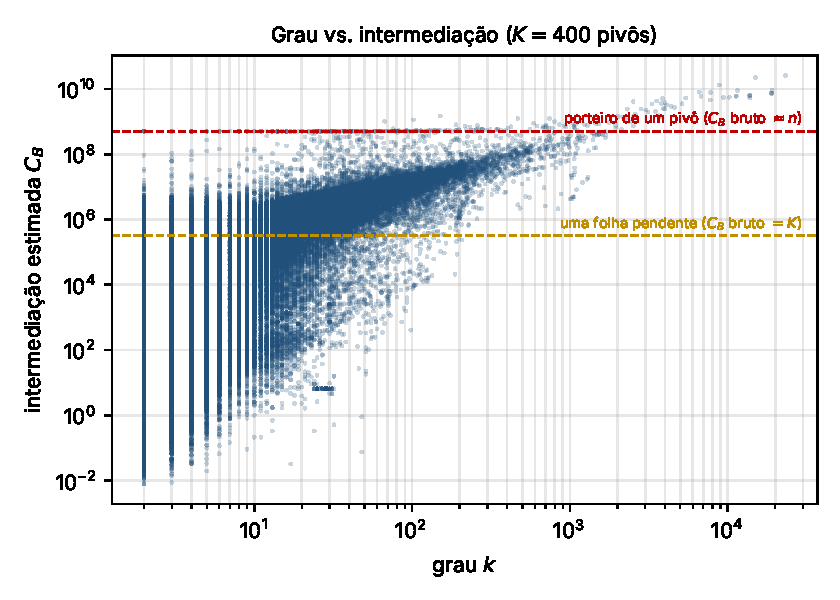
\includegraphics[width=0.95\columnwidth]{../figuras/fig_betweenness.pdf}
\caption{Grau \textit{vs.} intermediação estimada. A correlação de posto
entre os dois rankings é \btSpearman{}, alta mas longe de 1: a nuvem se
abre justamente nos graus intermediários.}
\label{fig:betweenness}
\end{figure}

\paragraph{Duas faixas horizontais, e o que elas revelam.} A
Figura~\ref{fig:betweenness} tem duas linhas horizontais nítidas, e vale
explicá-las porque uma delas é uma limitação do método, não uma
propriedade da rede.

A linha de baixo, em $C_B$ bruto $=K$, reúne \btFolhas{} vértices e é
\emph{real}: um vértice que tem exatamente uma folha pendurada nele está
no caminho mínimo de todo mundo até essa folha, e portanto recebe
dependência~1 de cada um dos $K$ pivôs. A estimativa está correta.

A linha de cima, em $C_B$ bruto $\approx n$, é \emph{artefato da
amostragem}. São \btPorteiros{} vértices cuja razão
$C_B^{\text{bruto}}/n$ tem mediana \btPorteirosRazao{}: cada um deles é o
único caminho entre um pivô sorteado e o resto do grafo, e por isso
recebe de uma só vez uma dependência de ordem $n$. Em um cálculo exato
esses vértices também teriam intermediação, mas diluída entre todas as
fontes; com $K$ pivôs ela aparece concentrada em um pico. É a variância
do estimador se manifestando na periferia --- zero na maioria das vezes,
um salto grande quando um pivô cai atrás do vértice. Pelo mesmo motivo,
\btZeros{}\% dos vértices recebem estimativa exatamente zero.

O impacto prático sobre o ataque é pequeno, e dá para medi-lo: esses
\btPorteiros{} vértices são \btPorteirosPct{}\% dos \robR{} removidos, e
o corte dos 5\% mais centrais está em $C_B = \btCorte{}$, cerca de
\btFatorCorte{} vezes abaixo da faixa --- ou seja, o topo do
\textit{ranking}, que é o que determina o ataque, está muito acima da
região em que o ruído do estimador pesa. Ainda assim, registra-se a
limitação: o ranking de intermediação aqui é confiável no topo e ruidoso
na cauda.

\paragraph{Resultado do ataque, e uma surpresa.} Os dois conjuntos
atacados têm \btSobreposicao{}\% de sobreposição e correlação de posto
\btSpearman{}, mas produzem danos \emph{qualitativamente diferentes}
(Tabela~\ref{tab:ataquebt}):

\begin{itemize}[nosep]
  \item remover os 5\% de maior \textbf{grau} deixa $S=\btGrauS{}$, com
        caminho médio \btGrauL{} e diâmetro \btGrauDiam{} no que sobra;
  \item remover os 5\% de maior \textbf{intermediação} deixa
        $S=\btS{}$ --- \btRazaoS{} vezes \emph{mais} ---, mas com
        caminho médio \btL{} e diâmetro \btDiam{}, menos da metade.
\end{itemize}

\noindent
Ou seja: contra a intuição, o ataque por intermediação é \emph{menos}
destrutivo para o tamanho da componente gigante, embora isole mais
vértices (\btIso{}\% contra \btGrauIso{}\%). A leitura é que as duas
centralidades atacam partes distintas da rede. O grau remove o núcleo
dos servidores de plataforma e estilhaça a rede em um resíduo grande,
porém esgarçado --- sobra uma componente de caminho médio \btGrauL{},
quase oito vezes o original. A intermediação remove as pontes
periféricas, isolando muito blog de grau baixo, mas preserva o núcleo
denso, que continua curto por dentro.

Para a pergunta do Apêndice~C --- a rede é vulnerável a ataques
dirigidos? --- a resposta não muda, e fica mais forte: por qualquer uma
das três centralidades testadas (grau, PageRank e intermediação), 5\%
dos vértices bem escolhidos derrubam a componente gigante de
\robSintacto{} para algo entre \robScentAbs{} e 65\,528 vértices,
enquanto 5\% sorteados ao acaso preservam \robSrandAbs{}.

\subsection{Comparação com modelos clássicos (extra)}
\label{sec:modelos}

\begin{table*}[t]
\centering
\caption{G106 comparado a três modelos clássicos com o mesmo $n$ e
aproximadamente o mesmo $m$ (Barabási--Albert e Watts--Strogatz só admitem
$m$ múltiplo de $n$, daí $\langle k\rangle = 4$ nos dois). O $\gamma$ da
última linha é um estimador comparativo grosseiro --- máxima
verossimilhança tomando como cauda os 5\% maiores graus ---, aplicado de
forma idêntica aos quatro grafos; ele não substitui a estimativa de
Clauset da Tabela~\ref{tab:leipotencia}, que escolhe $k_{min}$ pelo
critério de Kolmogorov--Smirnov.}
\label{tab:modelos}
\scriptsize
\begin{tabular}{lrrrr}
\hline
 & \textbf{G106 (real)} & \textbf{Erd\H{o}s--Rényi} & \textbf{Barabási--Albert} & \textbf{Watts--Strogatz} \\ \hline
Grau médio $\langle k\rangle$ & 4,797 & 4,797 & 4,000 & 4,000 \\
Grau máximo & 23\,196 & 19 & 807 & 9 \\
Clusterização média $C$ & 0,04502 & \ensuremath{1,1 \times 10^{-5}} & \ensuremath{4,6 \times 10^{-5}} & 0,37405 \\
Transitividade global & 0,00184 & \ensuremath{8,9 \times 10^{-6}} & \ensuremath{4,2 \times 10^{-5}} & 0,35556 \\
Caminho médio $L$ & 4,351 & 8,706 & 7,241 & 19,276 \\
Fração na comp.\ gigante & 0,9392 & 0,9915 & 1,0000 & 1,0000 \\
Assortatividade de grau & -0,1039 & -0,0008 & 0,0060 & -0,0003 \\
$\gamma$ (cauda 5\%) & 2,12 & 8,62 & 3,15 & 9,08 \\
\hline
\end{tabular}

\end{table*}

\begin{figure}[t]
\centering
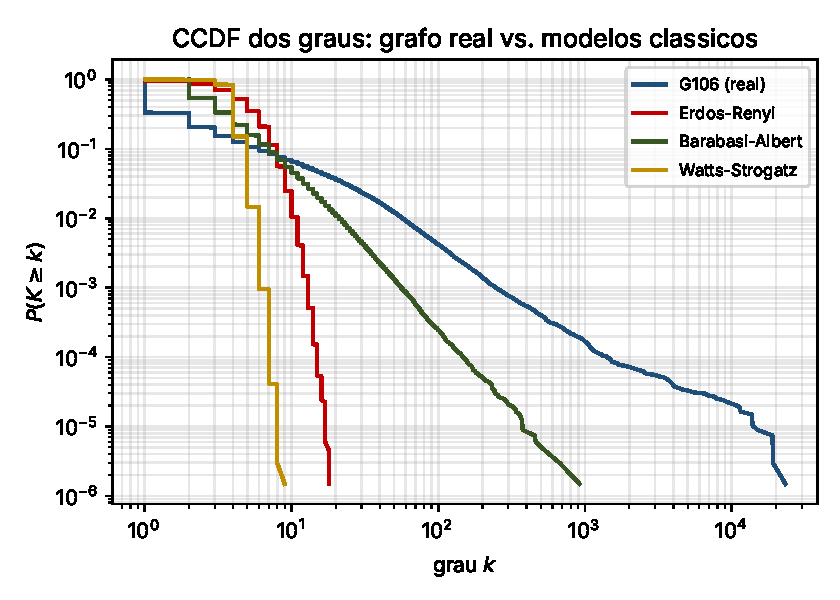
\includegraphics[width=0.6\columnwidth]{../figuras/fig_modelos.pdf}
\caption{CCDF dos graus: grafo real \textit{vs.} Erdős--Rényi,
Barabási--Albert e Watts--Strogatz.}
\label{fig:modelos}
\end{figure}

\paragraph{Resposta: de nenhum deles isoladamente, mas mais próximo de
Barabási--Albert.} Cada modelo captura uma propriedade e erra as outras:

\begin{itemize}[nosep]
  \item \textbf{Erdős--Rényi} acerta apenas a \emph{ordem de grandeza}
        das distâncias --- o seu caminho médio, \modErL{}, é quase o dobro
        do real (\swL{}), pois sem \textit{hubs} não há os atalhos que
        produzem o regime ultrapequeno. Erra grosseiramente a clusterização
        (\modErC{}, três ordens de grandeza abaixo) e a cauda, que é
        poissoniana (ver Figura~\ref{fig:modelos}).
  \item \textbf{Barabási--Albert} \cite{barabasi1999} é o que mais se
        aproxima: é o único dos três que reproduz a cauda pesada, e o seu
        caminho médio (\modBaL{}) fica mais perto do real que o de
        Erdős--Rényi --- ainda assim acima dele, em parte porque o modelo
        com $m=2$ gera menos arestas que o grafo real. A clusterização
        (\modBaC{}) continua cerca de mil vezes abaixo da real
        (\clusterMedia{}), porque a ligação preferencial pura não gera
        triângulos.
  \item \textbf{Watts--Strogatz} \cite{watts1998} é o único dos três a
        gerar agrupamento local forte, mas erra para o outro lado: a sua
        clusterização, \modWsC{}, é quase uma ordem de grandeza
        \emph{acima} da real (\clusterMedia{}). Além disso produz uma
        distribuição de graus quase homogênea, sem \textit{hubs}, e um
        caminho médio muito maior (\modWsL{}).
\end{itemize}

Há ainda um traço que \emph{nenhum} dos três reproduz: a assortatividade de
grau do grafo real é \modRealAssort{}, isto é, a rede é
\textbf{dissortativa} --- sites de grau alto ligam-se preferencialmente a
sites de grau baixo. Isso é típico de redes tecnológicas e de informação
(e oposto ao que se observa em redes sociais de pessoas) e decorre
diretamente da relação ``plataforma--usuário'' que domina esta rede.
Um modelo adequado precisaria combinar ligação preferencial com um
mecanismo gerador de triângulos e com essa dissortatividade --- por
exemplo, modelos de cópia de arestas ou de ligação preferencial com
fechamento triádico.

\subsection{A descoberta mais interessante}
\label{sec:descoberta}

A descoberta mais interessante está na Tabela~\ref{tab:hubs}:
\textbf{os maiores \textit{hubs} da blogosfera de 2008 não são veículos de
mídia nem blogs influentes --- são a infraestrutura técnica das
plataformas de blog}. Nove dos dez primeiros colocados são
\texttt{blogger.com} e os servidores de imagens
\texttt{1--4.bp.blogspot.com} e \texttt{bp0--3.blogger.com}; o único site
de \emph{conteúdo} entre eles --- e o primeiro a aparecer --- é
\texttt{en.wikipedia.org}, em sexto lugar.

Isso significa que a conectividade global desta rede --- o que a torna um
mundo pequeno e o que explica a sua fragilidade a ataques dirigidos --- é
sustentada em boa medida por \emph{artefatos de hospedagem}: cada post do
Blogger carrega imagens de um desses quatro servidores, e cada uma dessas
referências vira uma aresta. Dois blogs que nunca leram um ao outro ficam
a distância 2 porque ambos usam \texttt{2.bp.blogspot.com}.

A consequência metodológica é relevante e vale registrar com honestidade:
parte do efeito ``mundo pequeno'' medido na Seção~\ref{sec:smallworld} é
\emph{infraestrutural}, não editorial. Para separar os dois efeitos seria
necessário classificar os \textit{hostnames} em ``conteúdo'' e
``infraestrutura'' (CDNs, servidores de imagem, encurtadores, contadores de
acesso) e refazer a análise sobre o subgrafo editorial --- extensão
natural deste trabalho. O resultado também ilustra um ponto geral: em
análise de redes reais, \textbf{a definição do vértice é uma decisão
substantiva, não um detalhe técnico}; mudá-la muda a rede.

% =====================================================================
\section{Validação do recorte temporal}
\label{sec:validacaorecorte}

A objeção mais séria que se pode fazer a este trabalho é que todas as
conclusões vêm de uma janela de um mês: elas descrevem a blogosfera, ou
apenas agosto de 2008? Para responder, o pipeline inteiro --- da leitura
do arquivo bruto do SNAP até a análise de robustez, com exatamente os
mesmos tratamentos, algoritmos e sementes --- foi repetido sobre
\textbf{setembro de 2008} (\texttt{quotes\_2008-09.txt.gz}).

\begin{table}[t]
\centering
\caption{O mesmo pipeline aplicado a dois meses consecutivos. A coluna
de variação é relativa a agosto. Os valores de agosto nesta tabela foram
recalculados com $T=10$ repetições e a semente desta seção, e por isso
diferem na terceira casa dos da Seção~\ref{sec:robustez}.}
\label{tab:recorte}
\footnotesize
\begin{tabular}{lrrr}
\hline
\textbf{Grandeza} & \textbf{ago/2008} & \textbf{set/2008} & \textbf{variação} \\ \hline
Vértices $n$ & 673\,017 & 926\,946 & 37,7\% \\
Arestas $m$ & 1\,614\,246 & 2\,427\,184 & 50,4\% \\
Grau médio $\langle k\rangle$ & 4,797 & 5,237 & 9,2\% \\
Grau máximo & 23\,196 & 30\,236 & 30,4\% \\
Densidade & \ensuremath{7,1 \times 10^{-6}} & \ensuremath{5,6 \times 10^{-6}} & -20,7\% \\
Componentes conexas & 17\,265 & 23\,498 & 36,1\% \\
Fração na comp.\ gigante & 0,9392 & 0,9390 & -0,0\% \\
Clusterização média $C$ & 0,0450 & 0,0510 & 13,2\% \\
Diâmetro (exato) & 21 & 20 & -4,8\% \\
Raio (exato) & 11 & 10 & -9,1\% \\
Caminho médio $L$ & 4,322 & 4,536 & 4,9\% \\
Expoente $\gamma$ da cauda & 2,524 & 2,266 & -10,2\% \\
$S$ após remoção aleatória & 0,9132 & 0,9179 & 0,5\% \\
$S$ após ataque por grau & 0,0616 & 0,2127 & 245,3\% \\
\hline
\end{tabular}

\end{table}

\begin{figure}[t]
\centering
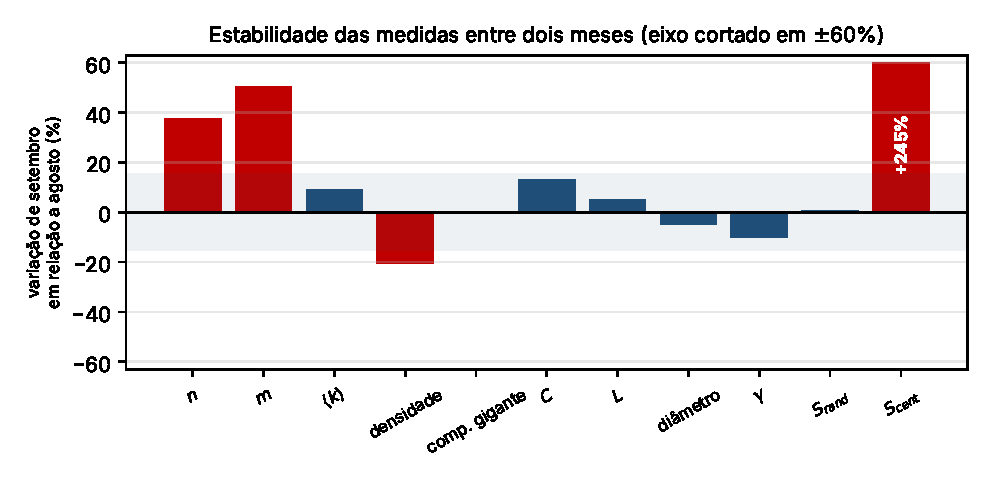
\includegraphics[width=\columnwidth]{../figuras/fig_recorte.pdf}
\caption{Variação percentual de cada grandeza entre os dois meses. A
faixa sombreada marca $\pm15\%$; em vermelho, as grandezas que saem
dela.}
\label{fig:recorte}
\end{figure}

\paragraph{Setembro é um mês maior, e por um motivo identificável.}
O grafo de setembro tem \setN{} vértices e \setM{} arestas ---
\setVarN{}\% e \setVarM{}\% a mais que agosto. Isso não é ruído de
amostragem: setembro de 2008 concentra a quebra do Lehman Brothers, no
dia 15, e a reta final da campanha presidencial norte-americana. Houve
mais publicação e mais linkagem. O teste, portanto, não é entre dois
meses equivalentes; é entre um mês comum e um mês de pico noticioso ---
o que o torna mais severo, não menos.

\paragraph{O que se mantém.} Apesar do salto de tamanho, as grandezas
das quais o relatório tira conclusões praticamente não se movem:

\begin{itemize}[nosep]
  \item a fração de vértices na componente gigante muda em
        \setVarCG{}\% --- de \fracCG{}\% para \setCG{}\%;
  \item o diâmetro vai de \diametro{} para \setDiam{} e o raio de
        \raio{} para \setRaio{}, ambos exatos;
  \item o caminho médio passa de \agoLdez{} para \setL{}
        (\setVarL{}\%), permanecendo pouco acima de~4 em um grafo que
        cresceu quase 40\%;
  \item o expoente da cauda vai de \plGamma{} para \setGamma{}
        (\setVarGamma{}\% de variação), permanecendo dentro da faixa
        $2<\gamma<3$ que sustenta toda a discussão da
        Seção~\ref{sec:leipotencia};
  \item a robustez a falhas aleatórias é praticamente idêntica:
        $S_{rand}$ passa de \agoSrandDez{} para \setSrand{}
        (\setVarSrand{}\%).
\end{itemize}

\noindent
As três assinaturas que o trabalho afirma ter encontrado --- mundo
pequeno, cauda pesada e tolerância a falhas aleatórias --- reaparecem
sem alteração qualitativa em um mês independente.

\paragraph{O que não se mantém, e que seria desonesto omitir.} Uma
grandeza se desloca muito: o tamanho da componente gigante \emph{após o
ataque dirigido}. Em agosto sobra $S_{cent} = \robScent{}$; em setembro,
\setScent{}. A rede de setembro continua sendo muito mais vulnerável ao
ataque do que à falha aleatória --- \setScent{} contra \setSrand{}, uma
razão de mais de quatro para um ---, mas o estrago absoluto é bem menor
que em agosto.

A explicação não está na concentração de arestas nos \textit{hubs}, que
é quase a mesma nos dois meses (\concAgo{}\% das pontas de aresta no
topo de 5\% em agosto, \concSet{}\% em setembro). Está, mais
provavelmente, na redundância do que sobra: o grau médio da componente
gigante de setembro é \grauMedioCGset{}, contra \grauMedioCG{} em
agosto, de modo que o esqueleto remanescente depois da remoção é mais
denso e se mantém conectado com mais facilidade. Registramos isso como a
explicação mais plausível, não como demonstração --- separar o efeito do
tamanho do efeito da densidade exigiria repetir o experimento com
subgrafos de setembro truncados ao tamanho de agosto, o que fica como
trabalho futuro.

\paragraph{Conclusão da validação.} O recorte de um mês é adequado para
tudo o que este relatório conclui em termos \emph{qualitativos} e para
as grandezas estruturais em termos quantitativos. Já o valor numérico do
dano causado por um ataque dirigido é específico da janela observada e
não deve ser extrapolado. Essa distinção substitui, com evidência, a
afirmação não verificada que constava da versão anterior deste trabalho.

% =====================================================================
\section{Discussão crítica}
\label{sec:discussao}

\paragraph{O que os recortes comprometem.} O recorte temporal de um mês
produz um grafo que é um \emph{instantâneo} da blogosfera, não a sua
história. Relações que só se manifestariam ao longo de meses aparecem como
ausentes, e sites que entraram na coleta em setembro simplesmente não
existem aqui. O efeito mais visível é a enorme quantidade de vértices de
grau~1: boa parte deles teria grau maior em uma janela mais longa. Isso
provavelmente \emph{superestima} o expoente $\gamma$ e \emph{subestima} a
clusterização. Em contrapartida, as conclusões qualitativas --- mundo
pequeno, cauda pesada, fragilidade assimétrica --- são robustas a esse
tipo de truncamento, por serem propriedades de ordens de grandeza, não de
valores precisos.

\paragraph{O que a agregação por \textit{hostname} comprometeu.} Como
discutido na Seção~\ref{sec:descoberta}, ela promove servidores de
infraestrutura a super-\textit{hubs}. Uma agregação por domínio
registrável seria pior ainda (fundiria milhões de blogs em um único
vértice \texttt{blogspot.com}); manter o nível de documento seria
computacionalmente proibitivo. O \textit{hostname} é o melhor compromisso
disponível, mas não é neutro.

\paragraph{O que foi estimado e por quê.} Apenas três quantidades não são
exatas: o comprimento médio dos caminhos, o coeficiente de clusterização
usado na Seção~\ref{sec:smallworld} (amostra de \swAmostraC{} vértices; o
valor exato está na Tabela~\ref{tab:estrutura}) e as distâncias nos
cenários de robustez. Todas vêm acompanhadas de intervalo de confiança, e
em todos os casos a largura do intervalo é pequena demais para alterar
qualquer conclusão. Diâmetro e raio, que costumam ser reportados como
estimativas em trabalhos sobre redes grandes, aqui são \textbf{exatos}.

\paragraph{Ameaças à validade.} (i) O \textit{Memetracker} coletava de uma
lista de sites monitorados; a amostra não é a Web inteira e tem viés
anglófono e jornalístico. (ii) Hiperlinks são apenas um dos canais de
difusão de informação; não há dados de audiência. (iii) A conversão
dirigido $\to$ não dirigido descarta a assimetria ``quem linka quem'',
reintroduzida parcialmente pela análise de componentes fortemente conexas.

% =====================================================================
\section{Conclusão}

A rede de hiperlinks entre sites da blogosfera de agosto de 2008,
construída a partir do grafo \textit{G106} (\texttt{memetracker9}) da
coleção SNAP, é um grafo de \numVertices{} vértices e \numArestas{} arestas
com as três assinaturas clássicas de uma rede de informação real:

\begin{enumerate}[nosep]
  \item \textbf{Mundo pequeno (na verdade, ultrapequeno):} caminho médio
        \swL{} e diâmetro \diametro{}, com clusterização \swRazaoCer{}
        vezes maior que a de um grafo aleatório equivalente
        ($\sigma = \swSigmaEr{}$) e distâncias ainda \emph{menores} que
        as dele. Contra o modelo de configuração, que preserva a sequência
        de graus, o excesso de agrupamento sobrevive, embora reduzido a
        $C/C_{conf} = \swRazaoCconf{}$.
  \item \textbf{Cauda pesada:} $\gamma = \plGamma \pm \plGammaErro$ acima
        de $k_{min} = \plKmin{}$, na faixa $2<\gamma<3$ em que a variância
        do grau diverge --- embora o teste formal de lei de potência pura
        seja rejeitado, como é regra em redes empíricas.
  \item \textbf{Robustez assimétrica:} tolerante a falhas aleatórias
        ($S=\robSrand{}$ após remover 5\% ao acaso) e frágil a ataques
        dirigidos, por qualquer das três centralidades testadas ---
        grau ($S=\robScent{}$), PageRank ($S=\robSpr{}$) e
        intermediação estimada por amostragem de pivôs ($S=\btS{}$).
\end{enumerate}

Do ponto de vista algorítmico, as implementações próprias reproduziram as
complexidades teóricas, e dois algoritmos do programa mostraram-se
inadequados à escala do problema por razões distintas e instrutivas:
Floyd--Warshall por custo cúbico em tempo e quadrático em memória, e
Bellman--Ford por ser desnecessário na ausência de pesos negativos. Em
compensação, um algoritmo que não estava no programa --- o
\textit{BoundingDiameters} --- permitiu obter diâmetro e raio
\emph{exatos} com \bfsDiametro{} buscas em largura, onde a abordagem
ingênua precisaria de \tamCG{}.

Essas três conclusões não dependem da janela escolhida: repetindo o
pipeline inteiro em setembro de 2008
(Seção~\ref{sec:validacaorecorte}), todas reaparecem, com a ressalva
---~documentada~--- de que o \emph{valor} do dano causado por um ataque
dirigido é específico do mês.

A descoberta que mais nos surpreendeu, porém, não é algorítmica: os
super-\textit{hubs} dessa rede são servidores de imagem de plataformas de
blog, e não veículos de mídia. É um lembrete de que a escolha do que conta
como vértice determina a rede que se analisa. A análise por intermediação
(Seção~\ref{sec:betweenness}) completa o quadro: quando se mede posição
de ponte em vez de volume de ligações, são a Wikipédia, o YouTube e o
Flickr que sobem ao topo --- os servidores de imagem concentram arestas,
mas não é por eles que a informação atravessa a rede.

% =====================================================================
\section{Repositório}
\label{sec:repositorio}

Código-fonte (scripts Python), conjunto de dados tratado, resultados em
JSON/CSV, figuras e o fonte \LaTeX{} deste relatório, com instruções de
execução no \texttt{README.md}:

\begin{center}
\fbox{\parbox{0.93\columnwidth}{\centering\small
\textbf{\url{https://github.com/leonecastro9-ui/tp2-grafos-snap-g106}}}}
\end{center}

% =====================================================================
\begin{thebibliography}{9}

\bibitem{barabasi1999}
Barabási, A.-L. and Albert, R. (1999).
\newblock Emergence of scaling in random networks.
\newblock \textit{Science}, 286(5439):509--512.

\bibitem{broder2000}
Broder, A., Kumar, R., Maghoul, F., Raghavan, P., Rajagopalan, S., Stata, R.,
Tomkins, A. and Wiener, J. (2000).
\newblock Graph structure in the Web.
\newblock \textit{Computer Networks}, 33(1--6):309--320.

\bibitem{clauset2009}
Clauset, A., Shalizi, C. R. and Newman, M. E. J. (2009).
\newblock Power-law distributions in empirical data.
\newblock \textit{SIAM Review}, 51(4):661--703.

\bibitem{leskovec2009}
Leskovec, J., Backstrom, L. and Kleinberg, J. (2009).
\newblock Meme-tracking and the dynamics of the news cycle.
\newblock In \textit{Proceedings of the 15th ACM SIGKDD International
Conference on Knowledge Discovery and Data Mining}, pages 497--506.

\bibitem{snap}
Leskovec, J. and Krevl, A. (2014).
\newblock SNAP Datasets: Stanford large network dataset collection.
\newblock \url{http://snap.stanford.edu/data}.

\bibitem{takes2011}
Takes, F. W. and Kosters, W. A. (2011).
\newblock Determining the diameter of small world networks.
\newblock In \textit{Proceedings of the 20th ACM International Conference
on Information and Knowledge Management}, pages 1191--1196.

\bibitem{watts1998}
Watts, D. J. and Strogatz, S. H. (1998).
\newblock Collective dynamics of `small-world' networks.
\newblock \textit{Nature}, 393(6684):440--442.

\end{thebibliography}

\end{document}
